%=========================================================================
% Start of first day on sequences
%=========================================================================
\preClass{Sequences}

\begin{problem}
  \item Write out the numbers given by $\frac{(-1)^n}{n}$ where $n=1$,
    2, 3, 4, and 5.
    \vfill
  \item Determine a formula, $f(n)$, that satisfies the following
    pattern.
    \begin{eqnarray*}
      f(1) & = & 1, \\
      f(2) & = & \frac{1}{4}, \\
      f(3) & = & \frac{1}{9}, \\
      f(4) & = & \frac{1}{16}.
    \end{eqnarray*}
    \vfill
\end{problem}


\actTitle{Sequences}

\begin{problem}
  \item The index of refraction, $n$, for a material is defined to be
  \begin{eqnarray*}
    n & = & \frac{c}{v},
  \end{eqnarray*}
  where $c$ is the speed of light in a vacuum and $v$ is the speed of light within the material.
  When a beam of light moves through one material with an index of refraction $n_1$ and then strikes a second material some of the light is reflected and some of the light passes through the material.
  The first material has an index of refraction given by $n_1$, and the second material has an index of refraction of $n_2$.

    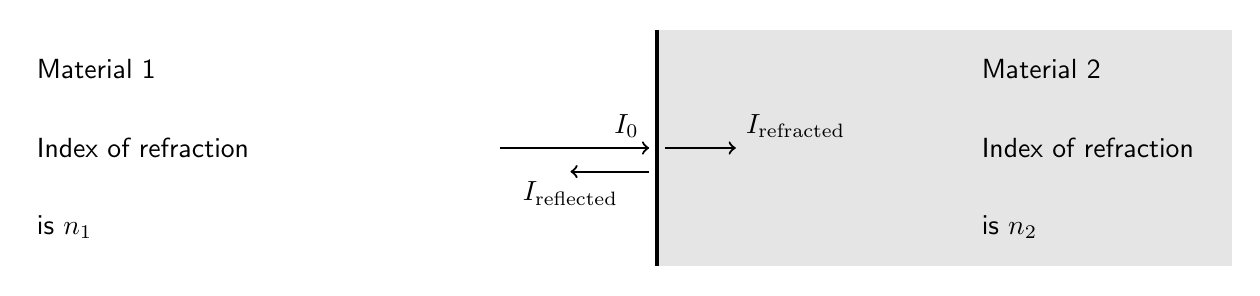
\begin{tikzpicture}[y=1.0cm,x=1.0cm,font=\sffamily]
    \node[anchor=west] at (0,2.0) {Material 1};
    \node[anchor=west] at (0,1.0) {Index of refraction};
    \node[anchor=west] at (0,0.0) {is $n_1$};

    \fill[gray!20!white] (8,-0.5) rectangle(15.3,2.5);
    \node[anchor=west] at (12,2.0) {Material 2};
    \node[anchor=west] at (12,1.0) {Index of refraction};
    \node[anchor=west] at (12,0.0) {is $n_2$};

    \draw[ultra thick,black] (8,-0.5) -- (8,2.5);
    \draw[thick,->] (6,1.0) -- (7.9,1.0) node[anchor=south east] {$I_0$};
    \draw[thick,->] (7.9,0.7) -- (6.9,0.7) node[anchor=north ] {$I_{\mathrm{reflected}}$};
    \draw[thick,->] (8.1,1.0) -- (9.0,1.0) node[anchor=south west] {$I_{\mathrm{refracted}}$};
    \end{tikzpicture}

  If the intensity of the original beam is $I_0$ then the intensity of the light reflected is
  \begin{eqnarray*}
    I_{\mathrm{reflected}} & = & \left(\frac{n_1-n_2}{n_1+n_2}\right)^2 I_0,
  \end{eqnarray*}

  A beam of light with intensity 1,000 N/C passes through air, $n_1=1$, and is moving from the left to the right.
  The beam hits the left face of a glass pane, $n_2=1.2$, that is perpendicular to the light beam.
  \begin{subproblem}
    \item  Determine the intensity of the light that is first reflected from the glass pane.
    \sideNote{Leave your answer as 1,000 times a fraction.}
    \vfill

    \item Determine the intensity of the light that is not reflected on the left face of the glass and continues inside the glass pane.
    \sideNote{Leave your answer as 1,000 times a fraction but do not simplify the fraction.}
      \vfill

      \clearpage

    \item When the beam of light strikes the other side, the right side, of the glass, part of that beam is reflected.
    Determine the intensity of the light that is reflected on the right side of the glass.
    \sideNote{Leave your answer as 1,000 times a fraction but do not simplify the fraction. The idea is to try and find the pattern.}
      \vfill

    \item The portion of the beam of light that is reflected back strikes the left side of the glass pane.
    Determine the intensity of the light that is reflected.

      \vfill

    \item This new light beam is reflected back to the right side of the glass pane.
    Determine the intensity of the light that is reflected.

      \vfill


    \item This new light beam is reflected back to the left side of the glass pane.
    Determine the intensity of the light that is reflected.

        \vfill

        \clearpage

    \item Assume that the original intensity of the light occurs at step 0.
    A new step is started each time the light is reflected from one of the sides of the pane of glass.
    Use the axes below to indicate the value of the intensity at each step starting at step 0.

      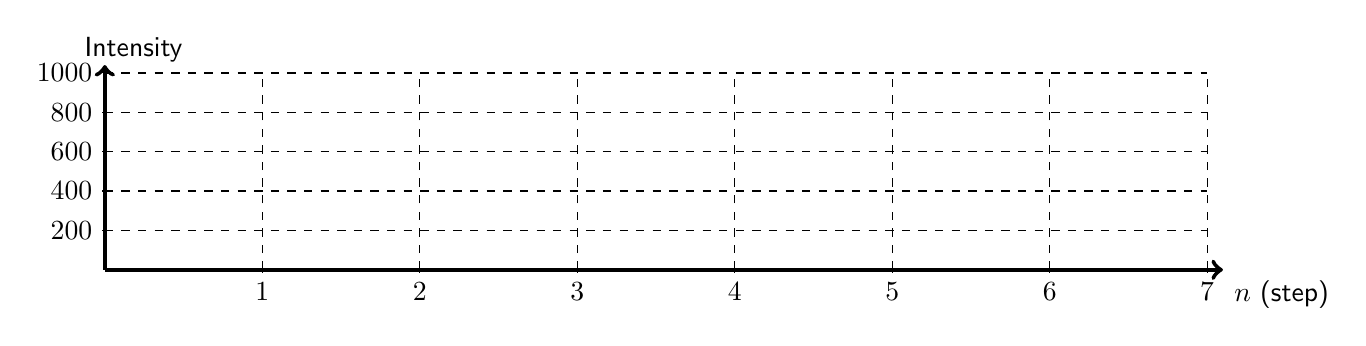
\begin{tikzpicture}[y=0.5cm, x=2.0cm,font=\sffamily]
        \begin{scope}[shift={(0,0)}]
          %% ticks
          \draw[xstep = 1, ystep=1,black,dashed] % very thin,opacity=0.85,
              (0.0, 0.0) grid ( 7.0, 5.0);
          %% axis
          \draw[ultra thick,->] (0,0) -- coordinate (x axis mid) (7.1,0)
               node[anchor = north west] {$n$ (step)};

          \draw[ultra thick,->] (0,0) -- coordinate (y axis mid) (0,5.2)
               node[anchor = south west,shift={(-0.2,-0.2)}] {Intensity};

          \foreach \y in {200,400,...,1000} {
            \draw (1pt, \y/200) -- (-1pt,\y/200) node[anchor = east] {$\y$}; }

          \foreach \x in {1,...,7} {
            \draw (\x,1pt) -- (\x,-1pt) node[anchor =north] {$\x$}; }

          %%\draw[thick] plot [smooth] coordinates { (0,-2) (0.5,-0.5) (1,0) (1.5,-0.5) (2,-1.5) (3,0) (4,2) (5,0) (6,-2)};

        \end{scope}

        \end{tikzpicture}

    \item What is happening with the value of the intensity after each step?
      \vfill

    \item After a large number of steps what will happen to the intensity?
      \vfill

    \item Determine a formula for the value of the intensity given the number of steps.
      \vfill

  \end{subproblem}

\clearpage
\item A sequence of numbers, $\left\{ a_n \right\}_{n=1}^\infty$, is
  given by
  \begin{eqnarray*}
    a_n & = & \frac{\cos(n)}{n}.
  \end{eqnarray*}
  Plot the numbers on the axes below. (Your calculator should be in radians mode.)

  %\scalebox{0.75}{%% Creator: Matplotlib, PGF backend
%%
%% To include the figure in your LaTeX document, write
%%   \input{<filename>.pgf}
%%
%% Make sure the required packages are loaded in your preamble
%%   \usepackage{pgf}
%%
%% Figures using additional raster images can only be included by \input if
%% they are in the same directory as the main LaTeX file. For loading figures
%% from other directories you can use the `import` package
%%   \usepackage{import}
%% and then include the figures with
%%   \import{<path to file>}{<filename>.pgf}
%%
%% Matplotlib used the following preamble
%%   \usepackage{fontspec}
%%   \setmainfont{Bitstream Vera Serif}
%%   \setsansfont{Bitstream Vera Sans}
%%   \setmonofont{Bitstream Vera Sans Mono}
%%
\begingroup%
\makeatletter%
\begin{pgfpicture}%
\pgfpathrectangle{\pgfpointorigin}{\pgfqpoint{8.000000in}{6.000000in}}%
\pgfusepath{use as bounding box, clip}%
\begin{pgfscope}%
\pgfsetbuttcap%
\pgfsetmiterjoin%
\definecolor{currentfill}{rgb}{1.000000,1.000000,1.000000}%
\pgfsetfillcolor{currentfill}%
\pgfsetlinewidth{0.000000pt}%
\definecolor{currentstroke}{rgb}{1.000000,1.000000,1.000000}%
\pgfsetstrokecolor{currentstroke}%
\pgfsetdash{}{0pt}%
\pgfpathmoveto{\pgfqpoint{0.000000in}{0.000000in}}%
\pgfpathlineto{\pgfqpoint{8.000000in}{0.000000in}}%
\pgfpathlineto{\pgfqpoint{8.000000in}{6.000000in}}%
\pgfpathlineto{\pgfqpoint{0.000000in}{6.000000in}}%
\pgfpathclose%
\pgfusepath{fill}%
\end{pgfscope}%
\begin{pgfscope}%
\pgfsetbuttcap%
\pgfsetmiterjoin%
\definecolor{currentfill}{rgb}{1.000000,1.000000,1.000000}%
\pgfsetfillcolor{currentfill}%
\pgfsetlinewidth{0.000000pt}%
\definecolor{currentstroke}{rgb}{0.000000,0.000000,0.000000}%
\pgfsetstrokecolor{currentstroke}%
\pgfsetstrokeopacity{0.000000}%
\pgfsetdash{}{0pt}%
\pgfpathmoveto{\pgfqpoint{1.000000in}{0.600000in}}%
\pgfpathlineto{\pgfqpoint{7.200000in}{0.600000in}}%
\pgfpathlineto{\pgfqpoint{7.200000in}{5.400000in}}%
\pgfpathlineto{\pgfqpoint{1.000000in}{5.400000in}}%
\pgfpathclose%
\pgfusepath{fill}%
\end{pgfscope}%
\begin{pgfscope}%
\pgfsetrectcap%
\pgfsetmiterjoin%
\pgfsetlinewidth{1.003750pt}%
\definecolor{currentstroke}{rgb}{0.000000,0.000000,0.000000}%
\pgfsetstrokecolor{currentstroke}%
\pgfsetdash{}{0pt}%
\pgfpathmoveto{\pgfqpoint{1.000000in}{5.400000in}}%
\pgfpathlineto{\pgfqpoint{7.200000in}{5.400000in}}%
\pgfusepath{stroke}%
\end{pgfscope}%
\begin{pgfscope}%
\pgfsetrectcap%
\pgfsetmiterjoin%
\pgfsetlinewidth{1.003750pt}%
\definecolor{currentstroke}{rgb}{0.000000,0.000000,0.000000}%
\pgfsetstrokecolor{currentstroke}%
\pgfsetdash{}{0pt}%
\pgfpathmoveto{\pgfqpoint{7.200000in}{0.600000in}}%
\pgfpathlineto{\pgfqpoint{7.200000in}{5.400000in}}%
\pgfusepath{stroke}%
\end{pgfscope}%
\begin{pgfscope}%
\pgfsetrectcap%
\pgfsetmiterjoin%
\pgfsetlinewidth{1.003750pt}%
\definecolor{currentstroke}{rgb}{0.000000,0.000000,0.000000}%
\pgfsetstrokecolor{currentstroke}%
\pgfsetdash{}{0pt}%
\pgfpathmoveto{\pgfqpoint{1.000000in}{0.600000in}}%
\pgfpathlineto{\pgfqpoint{7.200000in}{0.600000in}}%
\pgfusepath{stroke}%
\end{pgfscope}%
\begin{pgfscope}%
\pgfsetrectcap%
\pgfsetmiterjoin%
\pgfsetlinewidth{1.003750pt}%
\definecolor{currentstroke}{rgb}{0.000000,0.000000,0.000000}%
\pgfsetstrokecolor{currentstroke}%
\pgfsetdash{}{0pt}%
\pgfpathmoveto{\pgfqpoint{1.000000in}{0.600000in}}%
\pgfpathlineto{\pgfqpoint{1.000000in}{5.400000in}}%
\pgfusepath{stroke}%
\end{pgfscope}%
\begin{pgfscope}%
\pgfpathrectangle{\pgfqpoint{1.000000in}{0.600000in}}{\pgfqpoint{6.200000in}{4.800000in}} %
\pgfusepath{clip}%
\pgfsetbuttcap%
\pgfsetroundjoin%
\pgfsetlinewidth{0.301125pt}%
\definecolor{currentstroke}{rgb}{0.000000,0.000000,0.000000}%
\pgfsetstrokecolor{currentstroke}%
\pgfsetdash{{6.000000pt}{6.000000pt}}{0.000000pt}%
\pgfpathmoveto{\pgfqpoint{1.086111in}{0.600000in}}%
\pgfpathlineto{\pgfqpoint{1.086111in}{5.400000in}}%
\pgfusepath{stroke}%
\end{pgfscope}%
\begin{pgfscope}%
\pgfsetbuttcap%
\pgfsetroundjoin%
\definecolor{currentfill}{rgb}{0.000000,0.000000,0.000000}%
\pgfsetfillcolor{currentfill}%
\pgfsetlinewidth{0.501875pt}%
\definecolor{currentstroke}{rgb}{0.000000,0.000000,0.000000}%
\pgfsetstrokecolor{currentstroke}%
\pgfsetdash{}{0pt}%
\pgfsys@defobject{currentmarker}{\pgfqpoint{0.000000in}{0.000000in}}{\pgfqpoint{0.000000in}{0.055556in}}{%
\pgfpathmoveto{\pgfqpoint{0.000000in}{0.000000in}}%
\pgfpathlineto{\pgfqpoint{0.000000in}{0.055556in}}%
\pgfusepath{stroke,fill}%
}%
\begin{pgfscope}%
\pgfsys@transformshift{1.086111in}{0.600000in}%
\pgfsys@useobject{currentmarker}{}%
\end{pgfscope}%
\end{pgfscope}%
\begin{pgfscope}%
\pgfsetbuttcap%
\pgfsetroundjoin%
\definecolor{currentfill}{rgb}{0.000000,0.000000,0.000000}%
\pgfsetfillcolor{currentfill}%
\pgfsetlinewidth{0.501875pt}%
\definecolor{currentstroke}{rgb}{0.000000,0.000000,0.000000}%
\pgfsetstrokecolor{currentstroke}%
\pgfsetdash{}{0pt}%
\pgfsys@defobject{currentmarker}{\pgfqpoint{0.000000in}{-0.055556in}}{\pgfqpoint{0.000000in}{0.000000in}}{%
\pgfpathmoveto{\pgfqpoint{0.000000in}{0.000000in}}%
\pgfpathlineto{\pgfqpoint{0.000000in}{-0.055556in}}%
\pgfusepath{stroke,fill}%
}%
\begin{pgfscope}%
\pgfsys@transformshift{1.086111in}{5.400000in}%
\pgfsys@useobject{currentmarker}{}%
\end{pgfscope}%
\end{pgfscope}%
\begin{pgfscope}%
\pgftext[x=1.086111in,y=0.544444in,,top]{\sffamily\fontsize{12.000000}{14.400000}\selectfont \(\displaystyle 0\)}%
\end{pgfscope}%
\begin{pgfscope}%
\pgfpathrectangle{\pgfqpoint{1.000000in}{0.600000in}}{\pgfqpoint{6.200000in}{4.800000in}} %
\pgfusepath{clip}%
\pgfsetbuttcap%
\pgfsetroundjoin%
\pgfsetlinewidth{0.301125pt}%
\definecolor{currentstroke}{rgb}{0.000000,0.000000,0.000000}%
\pgfsetstrokecolor{currentstroke}%
\pgfsetdash{{6.000000pt}{6.000000pt}}{0.000000pt}%
\pgfpathmoveto{\pgfqpoint{1.947222in}{0.600000in}}%
\pgfpathlineto{\pgfqpoint{1.947222in}{5.400000in}}%
\pgfusepath{stroke}%
\end{pgfscope}%
\begin{pgfscope}%
\pgfsetbuttcap%
\pgfsetroundjoin%
\definecolor{currentfill}{rgb}{0.000000,0.000000,0.000000}%
\pgfsetfillcolor{currentfill}%
\pgfsetlinewidth{0.501875pt}%
\definecolor{currentstroke}{rgb}{0.000000,0.000000,0.000000}%
\pgfsetstrokecolor{currentstroke}%
\pgfsetdash{}{0pt}%
\pgfsys@defobject{currentmarker}{\pgfqpoint{0.000000in}{0.000000in}}{\pgfqpoint{0.000000in}{0.055556in}}{%
\pgfpathmoveto{\pgfqpoint{0.000000in}{0.000000in}}%
\pgfpathlineto{\pgfqpoint{0.000000in}{0.055556in}}%
\pgfusepath{stroke,fill}%
}%
\begin{pgfscope}%
\pgfsys@transformshift{1.947222in}{0.600000in}%
\pgfsys@useobject{currentmarker}{}%
\end{pgfscope}%
\end{pgfscope}%
\begin{pgfscope}%
\pgfsetbuttcap%
\pgfsetroundjoin%
\definecolor{currentfill}{rgb}{0.000000,0.000000,0.000000}%
\pgfsetfillcolor{currentfill}%
\pgfsetlinewidth{0.501875pt}%
\definecolor{currentstroke}{rgb}{0.000000,0.000000,0.000000}%
\pgfsetstrokecolor{currentstroke}%
\pgfsetdash{}{0pt}%
\pgfsys@defobject{currentmarker}{\pgfqpoint{0.000000in}{-0.055556in}}{\pgfqpoint{0.000000in}{0.000000in}}{%
\pgfpathmoveto{\pgfqpoint{0.000000in}{0.000000in}}%
\pgfpathlineto{\pgfqpoint{0.000000in}{-0.055556in}}%
\pgfusepath{stroke,fill}%
}%
\begin{pgfscope}%
\pgfsys@transformshift{1.947222in}{5.400000in}%
\pgfsys@useobject{currentmarker}{}%
\end{pgfscope}%
\end{pgfscope}%
\begin{pgfscope}%
\pgftext[x=1.947222in,y=0.544444in,,top]{\sffamily\fontsize{12.000000}{14.400000}\selectfont \(\displaystyle 1\)}%
\end{pgfscope}%
\begin{pgfscope}%
\pgfpathrectangle{\pgfqpoint{1.000000in}{0.600000in}}{\pgfqpoint{6.200000in}{4.800000in}} %
\pgfusepath{clip}%
\pgfsetbuttcap%
\pgfsetroundjoin%
\pgfsetlinewidth{0.301125pt}%
\definecolor{currentstroke}{rgb}{0.000000,0.000000,0.000000}%
\pgfsetstrokecolor{currentstroke}%
\pgfsetdash{{6.000000pt}{6.000000pt}}{0.000000pt}%
\pgfpathmoveto{\pgfqpoint{2.808333in}{0.600000in}}%
\pgfpathlineto{\pgfqpoint{2.808333in}{5.400000in}}%
\pgfusepath{stroke}%
\end{pgfscope}%
\begin{pgfscope}%
\pgfsetbuttcap%
\pgfsetroundjoin%
\definecolor{currentfill}{rgb}{0.000000,0.000000,0.000000}%
\pgfsetfillcolor{currentfill}%
\pgfsetlinewidth{0.501875pt}%
\definecolor{currentstroke}{rgb}{0.000000,0.000000,0.000000}%
\pgfsetstrokecolor{currentstroke}%
\pgfsetdash{}{0pt}%
\pgfsys@defobject{currentmarker}{\pgfqpoint{0.000000in}{0.000000in}}{\pgfqpoint{0.000000in}{0.055556in}}{%
\pgfpathmoveto{\pgfqpoint{0.000000in}{0.000000in}}%
\pgfpathlineto{\pgfqpoint{0.000000in}{0.055556in}}%
\pgfusepath{stroke,fill}%
}%
\begin{pgfscope}%
\pgfsys@transformshift{2.808333in}{0.600000in}%
\pgfsys@useobject{currentmarker}{}%
\end{pgfscope}%
\end{pgfscope}%
\begin{pgfscope}%
\pgfsetbuttcap%
\pgfsetroundjoin%
\definecolor{currentfill}{rgb}{0.000000,0.000000,0.000000}%
\pgfsetfillcolor{currentfill}%
\pgfsetlinewidth{0.501875pt}%
\definecolor{currentstroke}{rgb}{0.000000,0.000000,0.000000}%
\pgfsetstrokecolor{currentstroke}%
\pgfsetdash{}{0pt}%
\pgfsys@defobject{currentmarker}{\pgfqpoint{0.000000in}{-0.055556in}}{\pgfqpoint{0.000000in}{0.000000in}}{%
\pgfpathmoveto{\pgfqpoint{0.000000in}{0.000000in}}%
\pgfpathlineto{\pgfqpoint{0.000000in}{-0.055556in}}%
\pgfusepath{stroke,fill}%
}%
\begin{pgfscope}%
\pgfsys@transformshift{2.808333in}{5.400000in}%
\pgfsys@useobject{currentmarker}{}%
\end{pgfscope}%
\end{pgfscope}%
\begin{pgfscope}%
\pgftext[x=2.808333in,y=0.544444in,,top]{\sffamily\fontsize{12.000000}{14.400000}\selectfont \(\displaystyle 2\)}%
\end{pgfscope}%
\begin{pgfscope}%
\pgfpathrectangle{\pgfqpoint{1.000000in}{0.600000in}}{\pgfqpoint{6.200000in}{4.800000in}} %
\pgfusepath{clip}%
\pgfsetbuttcap%
\pgfsetroundjoin%
\pgfsetlinewidth{0.301125pt}%
\definecolor{currentstroke}{rgb}{0.000000,0.000000,0.000000}%
\pgfsetstrokecolor{currentstroke}%
\pgfsetdash{{6.000000pt}{6.000000pt}}{0.000000pt}%
\pgfpathmoveto{\pgfqpoint{3.669444in}{0.600000in}}%
\pgfpathlineto{\pgfqpoint{3.669444in}{5.400000in}}%
\pgfusepath{stroke}%
\end{pgfscope}%
\begin{pgfscope}%
\pgfsetbuttcap%
\pgfsetroundjoin%
\definecolor{currentfill}{rgb}{0.000000,0.000000,0.000000}%
\pgfsetfillcolor{currentfill}%
\pgfsetlinewidth{0.501875pt}%
\definecolor{currentstroke}{rgb}{0.000000,0.000000,0.000000}%
\pgfsetstrokecolor{currentstroke}%
\pgfsetdash{}{0pt}%
\pgfsys@defobject{currentmarker}{\pgfqpoint{0.000000in}{0.000000in}}{\pgfqpoint{0.000000in}{0.055556in}}{%
\pgfpathmoveto{\pgfqpoint{0.000000in}{0.000000in}}%
\pgfpathlineto{\pgfqpoint{0.000000in}{0.055556in}}%
\pgfusepath{stroke,fill}%
}%
\begin{pgfscope}%
\pgfsys@transformshift{3.669444in}{0.600000in}%
\pgfsys@useobject{currentmarker}{}%
\end{pgfscope}%
\end{pgfscope}%
\begin{pgfscope}%
\pgfsetbuttcap%
\pgfsetroundjoin%
\definecolor{currentfill}{rgb}{0.000000,0.000000,0.000000}%
\pgfsetfillcolor{currentfill}%
\pgfsetlinewidth{0.501875pt}%
\definecolor{currentstroke}{rgb}{0.000000,0.000000,0.000000}%
\pgfsetstrokecolor{currentstroke}%
\pgfsetdash{}{0pt}%
\pgfsys@defobject{currentmarker}{\pgfqpoint{0.000000in}{-0.055556in}}{\pgfqpoint{0.000000in}{0.000000in}}{%
\pgfpathmoveto{\pgfqpoint{0.000000in}{0.000000in}}%
\pgfpathlineto{\pgfqpoint{0.000000in}{-0.055556in}}%
\pgfusepath{stroke,fill}%
}%
\begin{pgfscope}%
\pgfsys@transformshift{3.669444in}{5.400000in}%
\pgfsys@useobject{currentmarker}{}%
\end{pgfscope}%
\end{pgfscope}%
\begin{pgfscope}%
\pgftext[x=3.669444in,y=0.544444in,,top]{\sffamily\fontsize{12.000000}{14.400000}\selectfont \(\displaystyle 3\)}%
\end{pgfscope}%
\begin{pgfscope}%
\pgfpathrectangle{\pgfqpoint{1.000000in}{0.600000in}}{\pgfqpoint{6.200000in}{4.800000in}} %
\pgfusepath{clip}%
\pgfsetbuttcap%
\pgfsetroundjoin%
\pgfsetlinewidth{0.301125pt}%
\definecolor{currentstroke}{rgb}{0.000000,0.000000,0.000000}%
\pgfsetstrokecolor{currentstroke}%
\pgfsetdash{{6.000000pt}{6.000000pt}}{0.000000pt}%
\pgfpathmoveto{\pgfqpoint{4.530556in}{0.600000in}}%
\pgfpathlineto{\pgfqpoint{4.530556in}{5.400000in}}%
\pgfusepath{stroke}%
\end{pgfscope}%
\begin{pgfscope}%
\pgfsetbuttcap%
\pgfsetroundjoin%
\definecolor{currentfill}{rgb}{0.000000,0.000000,0.000000}%
\pgfsetfillcolor{currentfill}%
\pgfsetlinewidth{0.501875pt}%
\definecolor{currentstroke}{rgb}{0.000000,0.000000,0.000000}%
\pgfsetstrokecolor{currentstroke}%
\pgfsetdash{}{0pt}%
\pgfsys@defobject{currentmarker}{\pgfqpoint{0.000000in}{0.000000in}}{\pgfqpoint{0.000000in}{0.055556in}}{%
\pgfpathmoveto{\pgfqpoint{0.000000in}{0.000000in}}%
\pgfpathlineto{\pgfqpoint{0.000000in}{0.055556in}}%
\pgfusepath{stroke,fill}%
}%
\begin{pgfscope}%
\pgfsys@transformshift{4.530556in}{0.600000in}%
\pgfsys@useobject{currentmarker}{}%
\end{pgfscope}%
\end{pgfscope}%
\begin{pgfscope}%
\pgfsetbuttcap%
\pgfsetroundjoin%
\definecolor{currentfill}{rgb}{0.000000,0.000000,0.000000}%
\pgfsetfillcolor{currentfill}%
\pgfsetlinewidth{0.501875pt}%
\definecolor{currentstroke}{rgb}{0.000000,0.000000,0.000000}%
\pgfsetstrokecolor{currentstroke}%
\pgfsetdash{}{0pt}%
\pgfsys@defobject{currentmarker}{\pgfqpoint{0.000000in}{-0.055556in}}{\pgfqpoint{0.000000in}{0.000000in}}{%
\pgfpathmoveto{\pgfqpoint{0.000000in}{0.000000in}}%
\pgfpathlineto{\pgfqpoint{0.000000in}{-0.055556in}}%
\pgfusepath{stroke,fill}%
}%
\begin{pgfscope}%
\pgfsys@transformshift{4.530556in}{5.400000in}%
\pgfsys@useobject{currentmarker}{}%
\end{pgfscope}%
\end{pgfscope}%
\begin{pgfscope}%
\pgftext[x=4.530556in,y=0.544444in,,top]{\sffamily\fontsize{12.000000}{14.400000}\selectfont \(\displaystyle 4\)}%
\end{pgfscope}%
\begin{pgfscope}%
\pgfpathrectangle{\pgfqpoint{1.000000in}{0.600000in}}{\pgfqpoint{6.200000in}{4.800000in}} %
\pgfusepath{clip}%
\pgfsetbuttcap%
\pgfsetroundjoin%
\pgfsetlinewidth{0.301125pt}%
\definecolor{currentstroke}{rgb}{0.000000,0.000000,0.000000}%
\pgfsetstrokecolor{currentstroke}%
\pgfsetdash{{6.000000pt}{6.000000pt}}{0.000000pt}%
\pgfpathmoveto{\pgfqpoint{5.391667in}{0.600000in}}%
\pgfpathlineto{\pgfqpoint{5.391667in}{5.400000in}}%
\pgfusepath{stroke}%
\end{pgfscope}%
\begin{pgfscope}%
\pgfsetbuttcap%
\pgfsetroundjoin%
\definecolor{currentfill}{rgb}{0.000000,0.000000,0.000000}%
\pgfsetfillcolor{currentfill}%
\pgfsetlinewidth{0.501875pt}%
\definecolor{currentstroke}{rgb}{0.000000,0.000000,0.000000}%
\pgfsetstrokecolor{currentstroke}%
\pgfsetdash{}{0pt}%
\pgfsys@defobject{currentmarker}{\pgfqpoint{0.000000in}{0.000000in}}{\pgfqpoint{0.000000in}{0.055556in}}{%
\pgfpathmoveto{\pgfqpoint{0.000000in}{0.000000in}}%
\pgfpathlineto{\pgfqpoint{0.000000in}{0.055556in}}%
\pgfusepath{stroke,fill}%
}%
\begin{pgfscope}%
\pgfsys@transformshift{5.391667in}{0.600000in}%
\pgfsys@useobject{currentmarker}{}%
\end{pgfscope}%
\end{pgfscope}%
\begin{pgfscope}%
\pgfsetbuttcap%
\pgfsetroundjoin%
\definecolor{currentfill}{rgb}{0.000000,0.000000,0.000000}%
\pgfsetfillcolor{currentfill}%
\pgfsetlinewidth{0.501875pt}%
\definecolor{currentstroke}{rgb}{0.000000,0.000000,0.000000}%
\pgfsetstrokecolor{currentstroke}%
\pgfsetdash{}{0pt}%
\pgfsys@defobject{currentmarker}{\pgfqpoint{0.000000in}{-0.055556in}}{\pgfqpoint{0.000000in}{0.000000in}}{%
\pgfpathmoveto{\pgfqpoint{0.000000in}{0.000000in}}%
\pgfpathlineto{\pgfqpoint{0.000000in}{-0.055556in}}%
\pgfusepath{stroke,fill}%
}%
\begin{pgfscope}%
\pgfsys@transformshift{5.391667in}{5.400000in}%
\pgfsys@useobject{currentmarker}{}%
\end{pgfscope}%
\end{pgfscope}%
\begin{pgfscope}%
\pgftext[x=5.391667in,y=0.544444in,,top]{\sffamily\fontsize{12.000000}{14.400000}\selectfont \(\displaystyle 5\)}%
\end{pgfscope}%
\begin{pgfscope}%
\pgfpathrectangle{\pgfqpoint{1.000000in}{0.600000in}}{\pgfqpoint{6.200000in}{4.800000in}} %
\pgfusepath{clip}%
\pgfsetbuttcap%
\pgfsetroundjoin%
\pgfsetlinewidth{0.301125pt}%
\definecolor{currentstroke}{rgb}{0.000000,0.000000,0.000000}%
\pgfsetstrokecolor{currentstroke}%
\pgfsetdash{{6.000000pt}{6.000000pt}}{0.000000pt}%
\pgfpathmoveto{\pgfqpoint{6.252778in}{0.600000in}}%
\pgfpathlineto{\pgfqpoint{6.252778in}{5.400000in}}%
\pgfusepath{stroke}%
\end{pgfscope}%
\begin{pgfscope}%
\pgfsetbuttcap%
\pgfsetroundjoin%
\definecolor{currentfill}{rgb}{0.000000,0.000000,0.000000}%
\pgfsetfillcolor{currentfill}%
\pgfsetlinewidth{0.501875pt}%
\definecolor{currentstroke}{rgb}{0.000000,0.000000,0.000000}%
\pgfsetstrokecolor{currentstroke}%
\pgfsetdash{}{0pt}%
\pgfsys@defobject{currentmarker}{\pgfqpoint{0.000000in}{0.000000in}}{\pgfqpoint{0.000000in}{0.055556in}}{%
\pgfpathmoveto{\pgfqpoint{0.000000in}{0.000000in}}%
\pgfpathlineto{\pgfqpoint{0.000000in}{0.055556in}}%
\pgfusepath{stroke,fill}%
}%
\begin{pgfscope}%
\pgfsys@transformshift{6.252778in}{0.600000in}%
\pgfsys@useobject{currentmarker}{}%
\end{pgfscope}%
\end{pgfscope}%
\begin{pgfscope}%
\pgfsetbuttcap%
\pgfsetroundjoin%
\definecolor{currentfill}{rgb}{0.000000,0.000000,0.000000}%
\pgfsetfillcolor{currentfill}%
\pgfsetlinewidth{0.501875pt}%
\definecolor{currentstroke}{rgb}{0.000000,0.000000,0.000000}%
\pgfsetstrokecolor{currentstroke}%
\pgfsetdash{}{0pt}%
\pgfsys@defobject{currentmarker}{\pgfqpoint{0.000000in}{-0.055556in}}{\pgfqpoint{0.000000in}{0.000000in}}{%
\pgfpathmoveto{\pgfqpoint{0.000000in}{0.000000in}}%
\pgfpathlineto{\pgfqpoint{0.000000in}{-0.055556in}}%
\pgfusepath{stroke,fill}%
}%
\begin{pgfscope}%
\pgfsys@transformshift{6.252778in}{5.400000in}%
\pgfsys@useobject{currentmarker}{}%
\end{pgfscope}%
\end{pgfscope}%
\begin{pgfscope}%
\pgftext[x=6.252778in,y=0.544444in,,top]{\sffamily\fontsize{12.000000}{14.400000}\selectfont \(\displaystyle 6\)}%
\end{pgfscope}%
\begin{pgfscope}%
\pgfpathrectangle{\pgfqpoint{1.000000in}{0.600000in}}{\pgfqpoint{6.200000in}{4.800000in}} %
\pgfusepath{clip}%
\pgfsetbuttcap%
\pgfsetroundjoin%
\pgfsetlinewidth{0.301125pt}%
\definecolor{currentstroke}{rgb}{0.000000,0.000000,0.000000}%
\pgfsetstrokecolor{currentstroke}%
\pgfsetdash{{6.000000pt}{6.000000pt}}{0.000000pt}%
\pgfpathmoveto{\pgfqpoint{7.113889in}{0.600000in}}%
\pgfpathlineto{\pgfqpoint{7.113889in}{5.400000in}}%
\pgfusepath{stroke}%
\end{pgfscope}%
\begin{pgfscope}%
\pgfsetbuttcap%
\pgfsetroundjoin%
\definecolor{currentfill}{rgb}{0.000000,0.000000,0.000000}%
\pgfsetfillcolor{currentfill}%
\pgfsetlinewidth{0.501875pt}%
\definecolor{currentstroke}{rgb}{0.000000,0.000000,0.000000}%
\pgfsetstrokecolor{currentstroke}%
\pgfsetdash{}{0pt}%
\pgfsys@defobject{currentmarker}{\pgfqpoint{0.000000in}{0.000000in}}{\pgfqpoint{0.000000in}{0.055556in}}{%
\pgfpathmoveto{\pgfqpoint{0.000000in}{0.000000in}}%
\pgfpathlineto{\pgfqpoint{0.000000in}{0.055556in}}%
\pgfusepath{stroke,fill}%
}%
\begin{pgfscope}%
\pgfsys@transformshift{7.113889in}{0.600000in}%
\pgfsys@useobject{currentmarker}{}%
\end{pgfscope}%
\end{pgfscope}%
\begin{pgfscope}%
\pgfsetbuttcap%
\pgfsetroundjoin%
\definecolor{currentfill}{rgb}{0.000000,0.000000,0.000000}%
\pgfsetfillcolor{currentfill}%
\pgfsetlinewidth{0.501875pt}%
\definecolor{currentstroke}{rgb}{0.000000,0.000000,0.000000}%
\pgfsetstrokecolor{currentstroke}%
\pgfsetdash{}{0pt}%
\pgfsys@defobject{currentmarker}{\pgfqpoint{0.000000in}{-0.055556in}}{\pgfqpoint{0.000000in}{0.000000in}}{%
\pgfpathmoveto{\pgfqpoint{0.000000in}{0.000000in}}%
\pgfpathlineto{\pgfqpoint{0.000000in}{-0.055556in}}%
\pgfusepath{stroke,fill}%
}%
\begin{pgfscope}%
\pgfsys@transformshift{7.113889in}{5.400000in}%
\pgfsys@useobject{currentmarker}{}%
\end{pgfscope}%
\end{pgfscope}%
\begin{pgfscope}%
\pgftext[x=7.113889in,y=0.544444in,,top]{\sffamily\fontsize{12.000000}{14.400000}\selectfont \(\displaystyle 7\)}%
\end{pgfscope}%
\begin{pgfscope}%
\pgftext[x=4.100000in,y=0.313705in,,top]{\sffamily\fontsize{12.000000}{14.400000}\selectfont n}%
\end{pgfscope}%
\begin{pgfscope}%
\pgfpathrectangle{\pgfqpoint{1.000000in}{0.600000in}}{\pgfqpoint{6.200000in}{4.800000in}} %
\pgfusepath{clip}%
\pgfsetbuttcap%
\pgfsetroundjoin%
\pgfsetlinewidth{0.301125pt}%
\definecolor{currentstroke}{rgb}{0.000000,0.000000,0.000000}%
\pgfsetstrokecolor{currentstroke}%
\pgfsetdash{{6.000000pt}{6.000000pt}}{0.000000pt}%
\pgfpathmoveto{\pgfqpoint{1.000000in}{0.818182in}}%
\pgfpathlineto{\pgfqpoint{7.200000in}{0.818182in}}%
\pgfusepath{stroke}%
\end{pgfscope}%
\begin{pgfscope}%
\pgfsetbuttcap%
\pgfsetroundjoin%
\definecolor{currentfill}{rgb}{0.000000,0.000000,0.000000}%
\pgfsetfillcolor{currentfill}%
\pgfsetlinewidth{0.501875pt}%
\definecolor{currentstroke}{rgb}{0.000000,0.000000,0.000000}%
\pgfsetstrokecolor{currentstroke}%
\pgfsetdash{}{0pt}%
\pgfsys@defobject{currentmarker}{\pgfqpoint{0.000000in}{0.000000in}}{\pgfqpoint{0.055556in}{0.000000in}}{%
\pgfpathmoveto{\pgfqpoint{0.000000in}{0.000000in}}%
\pgfpathlineto{\pgfqpoint{0.055556in}{0.000000in}}%
\pgfusepath{stroke,fill}%
}%
\begin{pgfscope}%
\pgfsys@transformshift{1.000000in}{0.818182in}%
\pgfsys@useobject{currentmarker}{}%
\end{pgfscope}%
\end{pgfscope}%
\begin{pgfscope}%
\pgfsetbuttcap%
\pgfsetroundjoin%
\definecolor{currentfill}{rgb}{0.000000,0.000000,0.000000}%
\pgfsetfillcolor{currentfill}%
\pgfsetlinewidth{0.501875pt}%
\definecolor{currentstroke}{rgb}{0.000000,0.000000,0.000000}%
\pgfsetstrokecolor{currentstroke}%
\pgfsetdash{}{0pt}%
\pgfsys@defobject{currentmarker}{\pgfqpoint{-0.055556in}{0.000000in}}{\pgfqpoint{0.000000in}{0.000000in}}{%
\pgfpathmoveto{\pgfqpoint{0.000000in}{0.000000in}}%
\pgfpathlineto{\pgfqpoint{-0.055556in}{0.000000in}}%
\pgfusepath{stroke,fill}%
}%
\begin{pgfscope}%
\pgfsys@transformshift{7.200000in}{0.818182in}%
\pgfsys@useobject{currentmarker}{}%
\end{pgfscope}%
\end{pgfscope}%
\begin{pgfscope}%
\pgftext[x=0.944444in,y=0.818182in,right,]{\sffamily\fontsize{12.000000}{14.400000}\selectfont \(\displaystyle -1.0\)}%
\end{pgfscope}%
\begin{pgfscope}%
\pgfpathrectangle{\pgfqpoint{1.000000in}{0.600000in}}{\pgfqpoint{6.200000in}{4.800000in}} %
\pgfusepath{clip}%
\pgfsetbuttcap%
\pgfsetroundjoin%
\pgfsetlinewidth{0.301125pt}%
\definecolor{currentstroke}{rgb}{0.000000,0.000000,0.000000}%
\pgfsetstrokecolor{currentstroke}%
\pgfsetdash{{6.000000pt}{6.000000pt}}{0.000000pt}%
\pgfpathmoveto{\pgfqpoint{1.000000in}{1.254545in}}%
\pgfpathlineto{\pgfqpoint{7.200000in}{1.254545in}}%
\pgfusepath{stroke}%
\end{pgfscope}%
\begin{pgfscope}%
\pgfsetbuttcap%
\pgfsetroundjoin%
\definecolor{currentfill}{rgb}{0.000000,0.000000,0.000000}%
\pgfsetfillcolor{currentfill}%
\pgfsetlinewidth{0.501875pt}%
\definecolor{currentstroke}{rgb}{0.000000,0.000000,0.000000}%
\pgfsetstrokecolor{currentstroke}%
\pgfsetdash{}{0pt}%
\pgfsys@defobject{currentmarker}{\pgfqpoint{0.000000in}{0.000000in}}{\pgfqpoint{0.055556in}{0.000000in}}{%
\pgfpathmoveto{\pgfqpoint{0.000000in}{0.000000in}}%
\pgfpathlineto{\pgfqpoint{0.055556in}{0.000000in}}%
\pgfusepath{stroke,fill}%
}%
\begin{pgfscope}%
\pgfsys@transformshift{1.000000in}{1.254545in}%
\pgfsys@useobject{currentmarker}{}%
\end{pgfscope}%
\end{pgfscope}%
\begin{pgfscope}%
\pgfsetbuttcap%
\pgfsetroundjoin%
\definecolor{currentfill}{rgb}{0.000000,0.000000,0.000000}%
\pgfsetfillcolor{currentfill}%
\pgfsetlinewidth{0.501875pt}%
\definecolor{currentstroke}{rgb}{0.000000,0.000000,0.000000}%
\pgfsetstrokecolor{currentstroke}%
\pgfsetdash{}{0pt}%
\pgfsys@defobject{currentmarker}{\pgfqpoint{-0.055556in}{0.000000in}}{\pgfqpoint{0.000000in}{0.000000in}}{%
\pgfpathmoveto{\pgfqpoint{0.000000in}{0.000000in}}%
\pgfpathlineto{\pgfqpoint{-0.055556in}{0.000000in}}%
\pgfusepath{stroke,fill}%
}%
\begin{pgfscope}%
\pgfsys@transformshift{7.200000in}{1.254545in}%
\pgfsys@useobject{currentmarker}{}%
\end{pgfscope}%
\end{pgfscope}%
\begin{pgfscope}%
\pgftext[x=0.944444in,y=1.254545in,right,]{\sffamily\fontsize{12.000000}{14.400000}\selectfont \(\displaystyle -0.8\)}%
\end{pgfscope}%
\begin{pgfscope}%
\pgfpathrectangle{\pgfqpoint{1.000000in}{0.600000in}}{\pgfqpoint{6.200000in}{4.800000in}} %
\pgfusepath{clip}%
\pgfsetbuttcap%
\pgfsetroundjoin%
\pgfsetlinewidth{0.301125pt}%
\definecolor{currentstroke}{rgb}{0.000000,0.000000,0.000000}%
\pgfsetstrokecolor{currentstroke}%
\pgfsetdash{{6.000000pt}{6.000000pt}}{0.000000pt}%
\pgfpathmoveto{\pgfqpoint{1.000000in}{1.690909in}}%
\pgfpathlineto{\pgfqpoint{7.200000in}{1.690909in}}%
\pgfusepath{stroke}%
\end{pgfscope}%
\begin{pgfscope}%
\pgfsetbuttcap%
\pgfsetroundjoin%
\definecolor{currentfill}{rgb}{0.000000,0.000000,0.000000}%
\pgfsetfillcolor{currentfill}%
\pgfsetlinewidth{0.501875pt}%
\definecolor{currentstroke}{rgb}{0.000000,0.000000,0.000000}%
\pgfsetstrokecolor{currentstroke}%
\pgfsetdash{}{0pt}%
\pgfsys@defobject{currentmarker}{\pgfqpoint{0.000000in}{0.000000in}}{\pgfqpoint{0.055556in}{0.000000in}}{%
\pgfpathmoveto{\pgfqpoint{0.000000in}{0.000000in}}%
\pgfpathlineto{\pgfqpoint{0.055556in}{0.000000in}}%
\pgfusepath{stroke,fill}%
}%
\begin{pgfscope}%
\pgfsys@transformshift{1.000000in}{1.690909in}%
\pgfsys@useobject{currentmarker}{}%
\end{pgfscope}%
\end{pgfscope}%
\begin{pgfscope}%
\pgfsetbuttcap%
\pgfsetroundjoin%
\definecolor{currentfill}{rgb}{0.000000,0.000000,0.000000}%
\pgfsetfillcolor{currentfill}%
\pgfsetlinewidth{0.501875pt}%
\definecolor{currentstroke}{rgb}{0.000000,0.000000,0.000000}%
\pgfsetstrokecolor{currentstroke}%
\pgfsetdash{}{0pt}%
\pgfsys@defobject{currentmarker}{\pgfqpoint{-0.055556in}{0.000000in}}{\pgfqpoint{0.000000in}{0.000000in}}{%
\pgfpathmoveto{\pgfqpoint{0.000000in}{0.000000in}}%
\pgfpathlineto{\pgfqpoint{-0.055556in}{0.000000in}}%
\pgfusepath{stroke,fill}%
}%
\begin{pgfscope}%
\pgfsys@transformshift{7.200000in}{1.690909in}%
\pgfsys@useobject{currentmarker}{}%
\end{pgfscope}%
\end{pgfscope}%
\begin{pgfscope}%
\pgftext[x=0.944444in,y=1.690909in,right,]{\sffamily\fontsize{12.000000}{14.400000}\selectfont \(\displaystyle -0.6\)}%
\end{pgfscope}%
\begin{pgfscope}%
\pgfpathrectangle{\pgfqpoint{1.000000in}{0.600000in}}{\pgfqpoint{6.200000in}{4.800000in}} %
\pgfusepath{clip}%
\pgfsetbuttcap%
\pgfsetroundjoin%
\pgfsetlinewidth{0.301125pt}%
\definecolor{currentstroke}{rgb}{0.000000,0.000000,0.000000}%
\pgfsetstrokecolor{currentstroke}%
\pgfsetdash{{6.000000pt}{6.000000pt}}{0.000000pt}%
\pgfpathmoveto{\pgfqpoint{1.000000in}{2.127273in}}%
\pgfpathlineto{\pgfqpoint{7.200000in}{2.127273in}}%
\pgfusepath{stroke}%
\end{pgfscope}%
\begin{pgfscope}%
\pgfsetbuttcap%
\pgfsetroundjoin%
\definecolor{currentfill}{rgb}{0.000000,0.000000,0.000000}%
\pgfsetfillcolor{currentfill}%
\pgfsetlinewidth{0.501875pt}%
\definecolor{currentstroke}{rgb}{0.000000,0.000000,0.000000}%
\pgfsetstrokecolor{currentstroke}%
\pgfsetdash{}{0pt}%
\pgfsys@defobject{currentmarker}{\pgfqpoint{0.000000in}{0.000000in}}{\pgfqpoint{0.055556in}{0.000000in}}{%
\pgfpathmoveto{\pgfqpoint{0.000000in}{0.000000in}}%
\pgfpathlineto{\pgfqpoint{0.055556in}{0.000000in}}%
\pgfusepath{stroke,fill}%
}%
\begin{pgfscope}%
\pgfsys@transformshift{1.000000in}{2.127273in}%
\pgfsys@useobject{currentmarker}{}%
\end{pgfscope}%
\end{pgfscope}%
\begin{pgfscope}%
\pgfsetbuttcap%
\pgfsetroundjoin%
\definecolor{currentfill}{rgb}{0.000000,0.000000,0.000000}%
\pgfsetfillcolor{currentfill}%
\pgfsetlinewidth{0.501875pt}%
\definecolor{currentstroke}{rgb}{0.000000,0.000000,0.000000}%
\pgfsetstrokecolor{currentstroke}%
\pgfsetdash{}{0pt}%
\pgfsys@defobject{currentmarker}{\pgfqpoint{-0.055556in}{0.000000in}}{\pgfqpoint{0.000000in}{0.000000in}}{%
\pgfpathmoveto{\pgfqpoint{0.000000in}{0.000000in}}%
\pgfpathlineto{\pgfqpoint{-0.055556in}{0.000000in}}%
\pgfusepath{stroke,fill}%
}%
\begin{pgfscope}%
\pgfsys@transformshift{7.200000in}{2.127273in}%
\pgfsys@useobject{currentmarker}{}%
\end{pgfscope}%
\end{pgfscope}%
\begin{pgfscope}%
\pgftext[x=0.944444in,y=2.127273in,right,]{\sffamily\fontsize{12.000000}{14.400000}\selectfont \(\displaystyle -0.4\)}%
\end{pgfscope}%
\begin{pgfscope}%
\pgfpathrectangle{\pgfqpoint{1.000000in}{0.600000in}}{\pgfqpoint{6.200000in}{4.800000in}} %
\pgfusepath{clip}%
\pgfsetbuttcap%
\pgfsetroundjoin%
\pgfsetlinewidth{0.301125pt}%
\definecolor{currentstroke}{rgb}{0.000000,0.000000,0.000000}%
\pgfsetstrokecolor{currentstroke}%
\pgfsetdash{{6.000000pt}{6.000000pt}}{0.000000pt}%
\pgfpathmoveto{\pgfqpoint{1.000000in}{2.563636in}}%
\pgfpathlineto{\pgfqpoint{7.200000in}{2.563636in}}%
\pgfusepath{stroke}%
\end{pgfscope}%
\begin{pgfscope}%
\pgfsetbuttcap%
\pgfsetroundjoin%
\definecolor{currentfill}{rgb}{0.000000,0.000000,0.000000}%
\pgfsetfillcolor{currentfill}%
\pgfsetlinewidth{0.501875pt}%
\definecolor{currentstroke}{rgb}{0.000000,0.000000,0.000000}%
\pgfsetstrokecolor{currentstroke}%
\pgfsetdash{}{0pt}%
\pgfsys@defobject{currentmarker}{\pgfqpoint{0.000000in}{0.000000in}}{\pgfqpoint{0.055556in}{0.000000in}}{%
\pgfpathmoveto{\pgfqpoint{0.000000in}{0.000000in}}%
\pgfpathlineto{\pgfqpoint{0.055556in}{0.000000in}}%
\pgfusepath{stroke,fill}%
}%
\begin{pgfscope}%
\pgfsys@transformshift{1.000000in}{2.563636in}%
\pgfsys@useobject{currentmarker}{}%
\end{pgfscope}%
\end{pgfscope}%
\begin{pgfscope}%
\pgfsetbuttcap%
\pgfsetroundjoin%
\definecolor{currentfill}{rgb}{0.000000,0.000000,0.000000}%
\pgfsetfillcolor{currentfill}%
\pgfsetlinewidth{0.501875pt}%
\definecolor{currentstroke}{rgb}{0.000000,0.000000,0.000000}%
\pgfsetstrokecolor{currentstroke}%
\pgfsetdash{}{0pt}%
\pgfsys@defobject{currentmarker}{\pgfqpoint{-0.055556in}{0.000000in}}{\pgfqpoint{0.000000in}{0.000000in}}{%
\pgfpathmoveto{\pgfqpoint{0.000000in}{0.000000in}}%
\pgfpathlineto{\pgfqpoint{-0.055556in}{0.000000in}}%
\pgfusepath{stroke,fill}%
}%
\begin{pgfscope}%
\pgfsys@transformshift{7.200000in}{2.563636in}%
\pgfsys@useobject{currentmarker}{}%
\end{pgfscope}%
\end{pgfscope}%
\begin{pgfscope}%
\pgftext[x=0.944444in,y=2.563636in,right,]{\sffamily\fontsize{12.000000}{14.400000}\selectfont \(\displaystyle -0.2\)}%
\end{pgfscope}%
\begin{pgfscope}%
\pgfpathrectangle{\pgfqpoint{1.000000in}{0.600000in}}{\pgfqpoint{6.200000in}{4.800000in}} %
\pgfusepath{clip}%
\pgfsetbuttcap%
\pgfsetroundjoin%
\pgfsetlinewidth{0.301125pt}%
\definecolor{currentstroke}{rgb}{0.000000,0.000000,0.000000}%
\pgfsetstrokecolor{currentstroke}%
\pgfsetdash{{6.000000pt}{6.000000pt}}{0.000000pt}%
\pgfpathmoveto{\pgfqpoint{1.000000in}{3.000000in}}%
\pgfpathlineto{\pgfqpoint{7.200000in}{3.000000in}}%
\pgfusepath{stroke}%
\end{pgfscope}%
\begin{pgfscope}%
\pgfsetbuttcap%
\pgfsetroundjoin%
\definecolor{currentfill}{rgb}{0.000000,0.000000,0.000000}%
\pgfsetfillcolor{currentfill}%
\pgfsetlinewidth{0.501875pt}%
\definecolor{currentstroke}{rgb}{0.000000,0.000000,0.000000}%
\pgfsetstrokecolor{currentstroke}%
\pgfsetdash{}{0pt}%
\pgfsys@defobject{currentmarker}{\pgfqpoint{0.000000in}{0.000000in}}{\pgfqpoint{0.055556in}{0.000000in}}{%
\pgfpathmoveto{\pgfqpoint{0.000000in}{0.000000in}}%
\pgfpathlineto{\pgfqpoint{0.055556in}{0.000000in}}%
\pgfusepath{stroke,fill}%
}%
\begin{pgfscope}%
\pgfsys@transformshift{1.000000in}{3.000000in}%
\pgfsys@useobject{currentmarker}{}%
\end{pgfscope}%
\end{pgfscope}%
\begin{pgfscope}%
\pgfsetbuttcap%
\pgfsetroundjoin%
\definecolor{currentfill}{rgb}{0.000000,0.000000,0.000000}%
\pgfsetfillcolor{currentfill}%
\pgfsetlinewidth{0.501875pt}%
\definecolor{currentstroke}{rgb}{0.000000,0.000000,0.000000}%
\pgfsetstrokecolor{currentstroke}%
\pgfsetdash{}{0pt}%
\pgfsys@defobject{currentmarker}{\pgfqpoint{-0.055556in}{0.000000in}}{\pgfqpoint{0.000000in}{0.000000in}}{%
\pgfpathmoveto{\pgfqpoint{0.000000in}{0.000000in}}%
\pgfpathlineto{\pgfqpoint{-0.055556in}{0.000000in}}%
\pgfusepath{stroke,fill}%
}%
\begin{pgfscope}%
\pgfsys@transformshift{7.200000in}{3.000000in}%
\pgfsys@useobject{currentmarker}{}%
\end{pgfscope}%
\end{pgfscope}%
\begin{pgfscope}%
\pgftext[x=0.944444in,y=3.000000in,right,]{\sffamily\fontsize{12.000000}{14.400000}\selectfont \(\displaystyle 0.0\)}%
\end{pgfscope}%
\begin{pgfscope}%
\pgfpathrectangle{\pgfqpoint{1.000000in}{0.600000in}}{\pgfqpoint{6.200000in}{4.800000in}} %
\pgfusepath{clip}%
\pgfsetbuttcap%
\pgfsetroundjoin%
\pgfsetlinewidth{0.301125pt}%
\definecolor{currentstroke}{rgb}{0.000000,0.000000,0.000000}%
\pgfsetstrokecolor{currentstroke}%
\pgfsetdash{{6.000000pt}{6.000000pt}}{0.000000pt}%
\pgfpathmoveto{\pgfqpoint{1.000000in}{3.436364in}}%
\pgfpathlineto{\pgfqpoint{7.200000in}{3.436364in}}%
\pgfusepath{stroke}%
\end{pgfscope}%
\begin{pgfscope}%
\pgfsetbuttcap%
\pgfsetroundjoin%
\definecolor{currentfill}{rgb}{0.000000,0.000000,0.000000}%
\pgfsetfillcolor{currentfill}%
\pgfsetlinewidth{0.501875pt}%
\definecolor{currentstroke}{rgb}{0.000000,0.000000,0.000000}%
\pgfsetstrokecolor{currentstroke}%
\pgfsetdash{}{0pt}%
\pgfsys@defobject{currentmarker}{\pgfqpoint{0.000000in}{0.000000in}}{\pgfqpoint{0.055556in}{0.000000in}}{%
\pgfpathmoveto{\pgfqpoint{0.000000in}{0.000000in}}%
\pgfpathlineto{\pgfqpoint{0.055556in}{0.000000in}}%
\pgfusepath{stroke,fill}%
}%
\begin{pgfscope}%
\pgfsys@transformshift{1.000000in}{3.436364in}%
\pgfsys@useobject{currentmarker}{}%
\end{pgfscope}%
\end{pgfscope}%
\begin{pgfscope}%
\pgfsetbuttcap%
\pgfsetroundjoin%
\definecolor{currentfill}{rgb}{0.000000,0.000000,0.000000}%
\pgfsetfillcolor{currentfill}%
\pgfsetlinewidth{0.501875pt}%
\definecolor{currentstroke}{rgb}{0.000000,0.000000,0.000000}%
\pgfsetstrokecolor{currentstroke}%
\pgfsetdash{}{0pt}%
\pgfsys@defobject{currentmarker}{\pgfqpoint{-0.055556in}{0.000000in}}{\pgfqpoint{0.000000in}{0.000000in}}{%
\pgfpathmoveto{\pgfqpoint{0.000000in}{0.000000in}}%
\pgfpathlineto{\pgfqpoint{-0.055556in}{0.000000in}}%
\pgfusepath{stroke,fill}%
}%
\begin{pgfscope}%
\pgfsys@transformshift{7.200000in}{3.436364in}%
\pgfsys@useobject{currentmarker}{}%
\end{pgfscope}%
\end{pgfscope}%
\begin{pgfscope}%
\pgftext[x=0.944444in,y=3.436364in,right,]{\sffamily\fontsize{12.000000}{14.400000}\selectfont \(\displaystyle 0.2\)}%
\end{pgfscope}%
\begin{pgfscope}%
\pgfpathrectangle{\pgfqpoint{1.000000in}{0.600000in}}{\pgfqpoint{6.200000in}{4.800000in}} %
\pgfusepath{clip}%
\pgfsetbuttcap%
\pgfsetroundjoin%
\pgfsetlinewidth{0.301125pt}%
\definecolor{currentstroke}{rgb}{0.000000,0.000000,0.000000}%
\pgfsetstrokecolor{currentstroke}%
\pgfsetdash{{6.000000pt}{6.000000pt}}{0.000000pt}%
\pgfpathmoveto{\pgfqpoint{1.000000in}{3.872727in}}%
\pgfpathlineto{\pgfqpoint{7.200000in}{3.872727in}}%
\pgfusepath{stroke}%
\end{pgfscope}%
\begin{pgfscope}%
\pgfsetbuttcap%
\pgfsetroundjoin%
\definecolor{currentfill}{rgb}{0.000000,0.000000,0.000000}%
\pgfsetfillcolor{currentfill}%
\pgfsetlinewidth{0.501875pt}%
\definecolor{currentstroke}{rgb}{0.000000,0.000000,0.000000}%
\pgfsetstrokecolor{currentstroke}%
\pgfsetdash{}{0pt}%
\pgfsys@defobject{currentmarker}{\pgfqpoint{0.000000in}{0.000000in}}{\pgfqpoint{0.055556in}{0.000000in}}{%
\pgfpathmoveto{\pgfqpoint{0.000000in}{0.000000in}}%
\pgfpathlineto{\pgfqpoint{0.055556in}{0.000000in}}%
\pgfusepath{stroke,fill}%
}%
\begin{pgfscope}%
\pgfsys@transformshift{1.000000in}{3.872727in}%
\pgfsys@useobject{currentmarker}{}%
\end{pgfscope}%
\end{pgfscope}%
\begin{pgfscope}%
\pgfsetbuttcap%
\pgfsetroundjoin%
\definecolor{currentfill}{rgb}{0.000000,0.000000,0.000000}%
\pgfsetfillcolor{currentfill}%
\pgfsetlinewidth{0.501875pt}%
\definecolor{currentstroke}{rgb}{0.000000,0.000000,0.000000}%
\pgfsetstrokecolor{currentstroke}%
\pgfsetdash{}{0pt}%
\pgfsys@defobject{currentmarker}{\pgfqpoint{-0.055556in}{0.000000in}}{\pgfqpoint{0.000000in}{0.000000in}}{%
\pgfpathmoveto{\pgfqpoint{0.000000in}{0.000000in}}%
\pgfpathlineto{\pgfqpoint{-0.055556in}{0.000000in}}%
\pgfusepath{stroke,fill}%
}%
\begin{pgfscope}%
\pgfsys@transformshift{7.200000in}{3.872727in}%
\pgfsys@useobject{currentmarker}{}%
\end{pgfscope}%
\end{pgfscope}%
\begin{pgfscope}%
\pgftext[x=0.944444in,y=3.872727in,right,]{\sffamily\fontsize{12.000000}{14.400000}\selectfont \(\displaystyle 0.4\)}%
\end{pgfscope}%
\begin{pgfscope}%
\pgfpathrectangle{\pgfqpoint{1.000000in}{0.600000in}}{\pgfqpoint{6.200000in}{4.800000in}} %
\pgfusepath{clip}%
\pgfsetbuttcap%
\pgfsetroundjoin%
\pgfsetlinewidth{0.301125pt}%
\definecolor{currentstroke}{rgb}{0.000000,0.000000,0.000000}%
\pgfsetstrokecolor{currentstroke}%
\pgfsetdash{{6.000000pt}{6.000000pt}}{0.000000pt}%
\pgfpathmoveto{\pgfqpoint{1.000000in}{4.309091in}}%
\pgfpathlineto{\pgfqpoint{7.200000in}{4.309091in}}%
\pgfusepath{stroke}%
\end{pgfscope}%
\begin{pgfscope}%
\pgfsetbuttcap%
\pgfsetroundjoin%
\definecolor{currentfill}{rgb}{0.000000,0.000000,0.000000}%
\pgfsetfillcolor{currentfill}%
\pgfsetlinewidth{0.501875pt}%
\definecolor{currentstroke}{rgb}{0.000000,0.000000,0.000000}%
\pgfsetstrokecolor{currentstroke}%
\pgfsetdash{}{0pt}%
\pgfsys@defobject{currentmarker}{\pgfqpoint{0.000000in}{0.000000in}}{\pgfqpoint{0.055556in}{0.000000in}}{%
\pgfpathmoveto{\pgfqpoint{0.000000in}{0.000000in}}%
\pgfpathlineto{\pgfqpoint{0.055556in}{0.000000in}}%
\pgfusepath{stroke,fill}%
}%
\begin{pgfscope}%
\pgfsys@transformshift{1.000000in}{4.309091in}%
\pgfsys@useobject{currentmarker}{}%
\end{pgfscope}%
\end{pgfscope}%
\begin{pgfscope}%
\pgfsetbuttcap%
\pgfsetroundjoin%
\definecolor{currentfill}{rgb}{0.000000,0.000000,0.000000}%
\pgfsetfillcolor{currentfill}%
\pgfsetlinewidth{0.501875pt}%
\definecolor{currentstroke}{rgb}{0.000000,0.000000,0.000000}%
\pgfsetstrokecolor{currentstroke}%
\pgfsetdash{}{0pt}%
\pgfsys@defobject{currentmarker}{\pgfqpoint{-0.055556in}{0.000000in}}{\pgfqpoint{0.000000in}{0.000000in}}{%
\pgfpathmoveto{\pgfqpoint{0.000000in}{0.000000in}}%
\pgfpathlineto{\pgfqpoint{-0.055556in}{0.000000in}}%
\pgfusepath{stroke,fill}%
}%
\begin{pgfscope}%
\pgfsys@transformshift{7.200000in}{4.309091in}%
\pgfsys@useobject{currentmarker}{}%
\end{pgfscope}%
\end{pgfscope}%
\begin{pgfscope}%
\pgftext[x=0.944444in,y=4.309091in,right,]{\sffamily\fontsize{12.000000}{14.400000}\selectfont \(\displaystyle 0.6\)}%
\end{pgfscope}%
\begin{pgfscope}%
\pgfpathrectangle{\pgfqpoint{1.000000in}{0.600000in}}{\pgfqpoint{6.200000in}{4.800000in}} %
\pgfusepath{clip}%
\pgfsetbuttcap%
\pgfsetroundjoin%
\pgfsetlinewidth{0.301125pt}%
\definecolor{currentstroke}{rgb}{0.000000,0.000000,0.000000}%
\pgfsetstrokecolor{currentstroke}%
\pgfsetdash{{6.000000pt}{6.000000pt}}{0.000000pt}%
\pgfpathmoveto{\pgfqpoint{1.000000in}{4.745455in}}%
\pgfpathlineto{\pgfqpoint{7.200000in}{4.745455in}}%
\pgfusepath{stroke}%
\end{pgfscope}%
\begin{pgfscope}%
\pgfsetbuttcap%
\pgfsetroundjoin%
\definecolor{currentfill}{rgb}{0.000000,0.000000,0.000000}%
\pgfsetfillcolor{currentfill}%
\pgfsetlinewidth{0.501875pt}%
\definecolor{currentstroke}{rgb}{0.000000,0.000000,0.000000}%
\pgfsetstrokecolor{currentstroke}%
\pgfsetdash{}{0pt}%
\pgfsys@defobject{currentmarker}{\pgfqpoint{0.000000in}{0.000000in}}{\pgfqpoint{0.055556in}{0.000000in}}{%
\pgfpathmoveto{\pgfqpoint{0.000000in}{0.000000in}}%
\pgfpathlineto{\pgfqpoint{0.055556in}{0.000000in}}%
\pgfusepath{stroke,fill}%
}%
\begin{pgfscope}%
\pgfsys@transformshift{1.000000in}{4.745455in}%
\pgfsys@useobject{currentmarker}{}%
\end{pgfscope}%
\end{pgfscope}%
\begin{pgfscope}%
\pgfsetbuttcap%
\pgfsetroundjoin%
\definecolor{currentfill}{rgb}{0.000000,0.000000,0.000000}%
\pgfsetfillcolor{currentfill}%
\pgfsetlinewidth{0.501875pt}%
\definecolor{currentstroke}{rgb}{0.000000,0.000000,0.000000}%
\pgfsetstrokecolor{currentstroke}%
\pgfsetdash{}{0pt}%
\pgfsys@defobject{currentmarker}{\pgfqpoint{-0.055556in}{0.000000in}}{\pgfqpoint{0.000000in}{0.000000in}}{%
\pgfpathmoveto{\pgfqpoint{0.000000in}{0.000000in}}%
\pgfpathlineto{\pgfqpoint{-0.055556in}{0.000000in}}%
\pgfusepath{stroke,fill}%
}%
\begin{pgfscope}%
\pgfsys@transformshift{7.200000in}{4.745455in}%
\pgfsys@useobject{currentmarker}{}%
\end{pgfscope}%
\end{pgfscope}%
\begin{pgfscope}%
\pgftext[x=0.944444in,y=4.745455in,right,]{\sffamily\fontsize{12.000000}{14.400000}\selectfont \(\displaystyle 0.8\)}%
\end{pgfscope}%
\begin{pgfscope}%
\pgfpathrectangle{\pgfqpoint{1.000000in}{0.600000in}}{\pgfqpoint{6.200000in}{4.800000in}} %
\pgfusepath{clip}%
\pgfsetbuttcap%
\pgfsetroundjoin%
\pgfsetlinewidth{0.301125pt}%
\definecolor{currentstroke}{rgb}{0.000000,0.000000,0.000000}%
\pgfsetstrokecolor{currentstroke}%
\pgfsetdash{{6.000000pt}{6.000000pt}}{0.000000pt}%
\pgfpathmoveto{\pgfqpoint{1.000000in}{5.181818in}}%
\pgfpathlineto{\pgfqpoint{7.200000in}{5.181818in}}%
\pgfusepath{stroke}%
\end{pgfscope}%
\begin{pgfscope}%
\pgfsetbuttcap%
\pgfsetroundjoin%
\definecolor{currentfill}{rgb}{0.000000,0.000000,0.000000}%
\pgfsetfillcolor{currentfill}%
\pgfsetlinewidth{0.501875pt}%
\definecolor{currentstroke}{rgb}{0.000000,0.000000,0.000000}%
\pgfsetstrokecolor{currentstroke}%
\pgfsetdash{}{0pt}%
\pgfsys@defobject{currentmarker}{\pgfqpoint{0.000000in}{0.000000in}}{\pgfqpoint{0.055556in}{0.000000in}}{%
\pgfpathmoveto{\pgfqpoint{0.000000in}{0.000000in}}%
\pgfpathlineto{\pgfqpoint{0.055556in}{0.000000in}}%
\pgfusepath{stroke,fill}%
}%
\begin{pgfscope}%
\pgfsys@transformshift{1.000000in}{5.181818in}%
\pgfsys@useobject{currentmarker}{}%
\end{pgfscope}%
\end{pgfscope}%
\begin{pgfscope}%
\pgfsetbuttcap%
\pgfsetroundjoin%
\definecolor{currentfill}{rgb}{0.000000,0.000000,0.000000}%
\pgfsetfillcolor{currentfill}%
\pgfsetlinewidth{0.501875pt}%
\definecolor{currentstroke}{rgb}{0.000000,0.000000,0.000000}%
\pgfsetstrokecolor{currentstroke}%
\pgfsetdash{}{0pt}%
\pgfsys@defobject{currentmarker}{\pgfqpoint{-0.055556in}{0.000000in}}{\pgfqpoint{0.000000in}{0.000000in}}{%
\pgfpathmoveto{\pgfqpoint{0.000000in}{0.000000in}}%
\pgfpathlineto{\pgfqpoint{-0.055556in}{0.000000in}}%
\pgfusepath{stroke,fill}%
}%
\begin{pgfscope}%
\pgfsys@transformshift{7.200000in}{5.181818in}%
\pgfsys@useobject{currentmarker}{}%
\end{pgfscope}%
\end{pgfscope}%
\begin{pgfscope}%
\pgftext[x=0.944444in,y=5.181818in,right,]{\sffamily\fontsize{12.000000}{14.400000}\selectfont \(\displaystyle 1.0\)}%
\end{pgfscope}%
\begin{pgfscope}%
\pgftext[x=0.536846in,y=3.000000in,,bottom,rotate=90.000000]{\sffamily\fontsize{12.000000}{14.400000}\selectfont $a_n$}%
\end{pgfscope}%
\begin{pgfscope}%
\pgftext[x=4.100000in,y=5.469444in,,base]{\sffamily\fontsize{14.400000}{17.280000}\selectfont Sequence}%
\end{pgfscope}%
\end{pgfpicture}%
\makeatother%
\endgroup%
}

  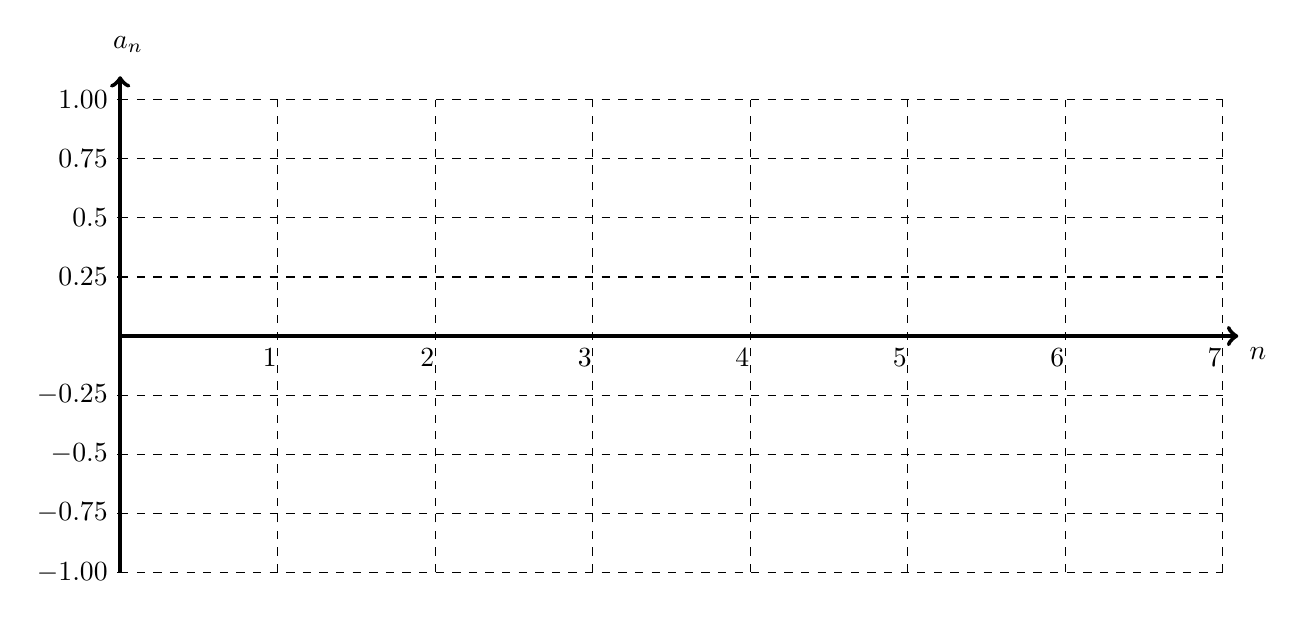
\begin{tikzpicture}[y=3.0cm, x=2.0cm,font=\sffamily]
    \begin{scope}[shift={(0,0)}]
      %% ticks
      \draw[xstep = 1, ystep=0.25,black,dashed] % very thin,opacity=0.85,
          (0.0, -1.0) grid ( 7.0, 1.0);
      %% axis
      \draw[ultra thick,->] (0,0) -- coordinate (x axis mid) (7.1,0)
           node[anchor = north west] {$n$};

      \draw[ultra thick,->] (0,-1) -- coordinate (y axis mid) (0,1.1)
           node[anchor = south,shift={(0.05,0.05)}] {$a_n$};

      \foreach \y in {-1.00,-0.75,-0.5,-0.25,0.25,0.5,0.75,1.00} {
        \draw (1pt, \y) -- (-1pt,\y) node[anchor = east] {$\y$}; }

      \foreach \x in {1,...,7} {
        \draw (\x,1pt) -- (\x,-1pt) node[anchor =north,shift={(-0.05,0)}] {$\x$}; }

      %%\draw[thick] plot [smooth] coordinates { (0,-2) (0.5,-0.5) (1,0) (1.5,-0.5) (2,-1.5) (3,0) (4,2) (5,0) (6,-2)};

    \end{scope}

    \end{tikzpicture}


  \begin{subproblem}
  \item Plot the numbers given by $b_n=\frac{1}{n}$ on the plot
    above.
  \item Plot the numbers given by $c_n=\frac{-1}{n}$ on the plot
    above.
  \item What is the relationship between $a_n$, $b_n$, and $c_n$?
    \vfill
  \item Determine the following limits
    \begin{eqnarray*}
      \lim_{n\rightarrow\infty} \frac{1}{n} & = & \\
      \lim_{n\rightarrow\infty} \frac{-1}{n} & = &
    \end{eqnarray*}
  \item What does this imply about the value of $a_n$ as $n$ gets large?
    Explain your reasoning.
    \vfill
  \end{subproblem}

  \clearpage

  \item For each part below determine value of $N$ that match the criteria.
  Assume that $n$ and $N$ are positive integers.
  \begin{subproblem}
    \item Determine a value of $N$ so that
    \begin{eqnarray*}
      \left| \frac{1}{n} - 0 \right| &  < 0.1
    \end{eqnarray*}
    for every $n>N$.

    \vfill

    \item Determine a value of $N$ so that
    \begin{eqnarray*}
      \left| \frac{1}{n} - 0 \right| &  < 0.01
    \end{eqnarray*}
    for every $n>N$.

    \vfill

    \item Determine a value of $N$ so that
    \begin{eqnarray*}
      \left| \frac{1}{n} - 0 \right| &  < \epsilon
    \end{eqnarray*}
    for every $n>N$ where $\epsilon>0$.

    \vfill

  \end{subproblem}
\end{problem}

\postClass

\begin{problem}
\item Briefly state two ideas from today's class.
  \begin{itemize}
  \item
  \item
  \end{itemize}
\item
  \begin{subproblem}
    \item
  \end{subproblem}
\end{problem}


%=========================================================================
% First day on series
%=========================================================================


\preClass{Series}

\begin{problem}
  \item Write out the numbers given by $\frac{1}{n}$ where $n=1$,
    2, 3, 4, and 5.
    \sideNote{This is called a sequence.}
    \vfill
  \item Determine the sum of the numbers in the previous problem.
    \sideNote{This is called a series.}
    \vfill
  \item Determine the value of the sum
    \begin{eqnarray*}
      \sum_{n=1}^{5} \frac{1}{n}.
    \end{eqnarray*}
\end{problem}


\actTitle{Series}

\begin{problem}
  \item We look at the intensity of light that is reflected within a pane of glass.

    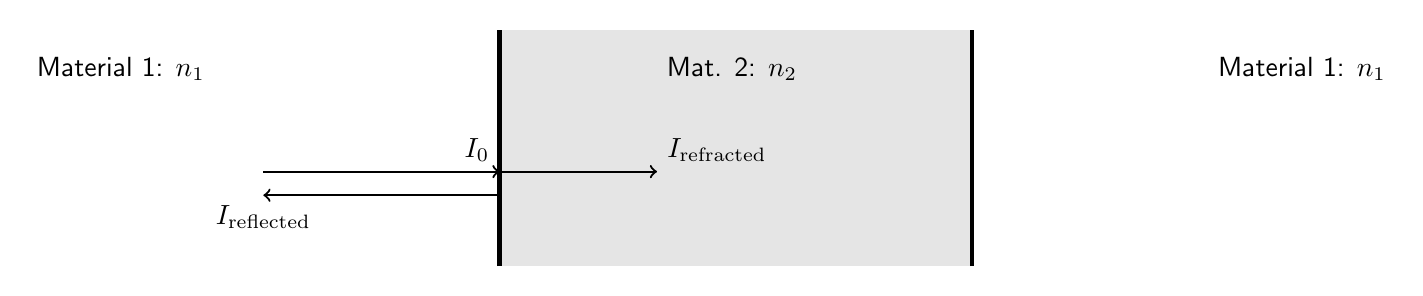
\begin{tikzpicture}[y=1.0cm,x=1.0cm,font=\sffamily]
    \node[anchor=west] at (0,2.0) {Material 1: $n_1$};
    \node[anchor=west] at (15,2.0) {Material 1: $n_1$};

    \fill[gray!20!white] (6,-0.5) rectangle(12,2.5);
    \node[anchor=west] at (8,2.0) {Mat. 2: $n_2$};

    \draw[ultra thick,black] (6,-0.5) -- (6,2.5);
    \draw[ultra thick,black] (12,-0.5) -- (12,2.5);
    \draw[thick,->] (3,0.7) -- (6,0.7) node[anchor=south east] {$I_0$};
    \draw[thick,->] (6,0.4) -- (3,0.4) node[anchor=north ] {$I_{\mathrm{reflected}}$};
    \draw[thick,->] (6,0.7) -- (8.0,0.7) node[anchor=south west] {$I_{\mathrm{refracted}}$};
    \end{tikzpicture}

  If the intensity of the original beam is $I_0$ then the intensity of the light reflected is
  \begin{eqnarray*}
    I_{\mathrm{reflected}} & = & \left(\frac{n_1-n_2}{n_1+n_2}\right)^2 I_0,
  \end{eqnarray*}

  A beam of light with intensity 1,000 N/C passes through air, $n_1=1$, and is moving from the left to the right.
  The beam hits the left face of a glass pane, $n_2=1.2$, that is perpendicular to the light beam.

  \begin{subproblem}
    \item  Determine the intensity of the light that is first reflected from the glass pane.
    \sideNote{Leave your answer as 1,000 times a fraction.}
    \vfill

    \item Determine the intensity of the light that is not reflected on the left face of the glass and continues inside the glass pane.
    \sideNote{Leave your answer as 1,000 times a fraction but do not simplify the fraction.}
      \vfill

      \clearpage

    \item When the beam of light strikes the other side, the right side, of the glass, part of that beam is reflected.
    Determine the intensity of the light that is reflected on the right side of the glass.
    Determine the sum of the light intensities within the glass after one internal bounce.
    \sideNote{Leave your answer as a sum that includes terms with 1,000 times a fraction but do not simplify the fractions. The idea is to try and find the pattern.}
      \vfill

    \item The portion of the beam of light that is reflected back strikes the left side of the glass pane.
    Determine the intensity of the light that is reflected.
    Determine the sum of the light intensities within the glass after two internal bounces.

      \vfill

    \item This new light beam is reflected back to the right side of the glass pane.
    Determine the intensity of the light that is reflected.
    Determine the sum of the light intensities within the glass after three internal bounces.

      \vfill


    \item This new light beam is reflected back to the left side of the glass pane.
    Determine the intensity of the light that is reflected.
    Determine the sum of the light intensities within the glass after four internal bounces.

        \vfill

        \clearpage

    \item Assume that the  intensity within the pane due to the first refracted beam of light occurs at step 0.
    A new step is started each time the light is reflected from one of the sides of the pane of glass.
    Use the axes below to indicate the value of the total intensity of light within the pane given the number of bounces.

      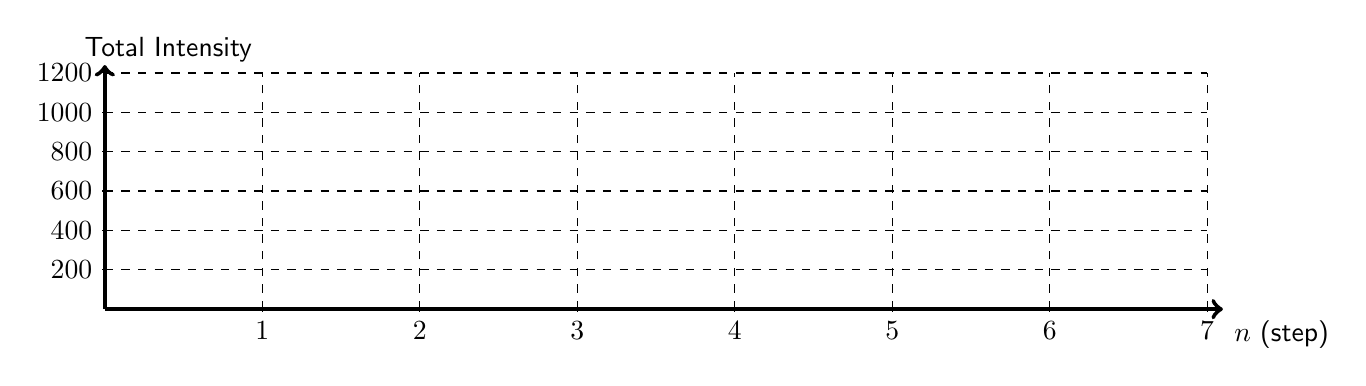
\begin{tikzpicture}[y=0.5cm, x=2.0cm,font=\sffamily]
        \begin{scope}[shift={(0,0)}]
          %% ticks
          \draw[xstep = 1, ystep=1,black,dashed] % very thin,opacity=0.85,
              (0.0, 0.0) grid ( 7.0, 6.0);
          %% axis
          \draw[ultra thick,->] (0,0) -- coordinate (x axis mid) (7.1,0)
               node[anchor = north west] {$n$ (step)};

          \draw[ultra thick,->] (0,0) -- coordinate (y axis mid) (0,6.2)
               node[anchor = south west,shift={(-0.2,-0.2)}] {Total Intensity};

          \foreach \y in {200,400,...,1200} {
            \draw (1pt, \y/200) -- (-1pt,\y/200) node[anchor = east] {$\y$}; }

          \foreach \x in {1,...,7} {
            \draw (\x,1pt) -- (\x,-1pt) node[anchor =north] {$\x$}; }

          %%\draw[thick] plot [smooth] coordinates { (0,-2) (0.5,-0.5) (1,0) (1.5,-0.5) (2,-1.5) (3,0) (4,2) (5,0) (6,-2)};

        \end{scope}

        \end{tikzpicture}

    \item What is happening with the value of the total intensity after each step?
      \vfill

    \item After a large number of steps what will happen to the total intensity?
      \vfill

    \item Show that the intensity after $N$ bounces, $S_N$, can be written in the form
    \begin{eqnarray*}
      S_N & = & A + A \cdot r + A \cdot r^2 + A \cdot r^3 + \cdots + A \cdot r^N.
    \end{eqnarray*}
    For this situation state the values of $A$ and $r$.
    \sideNote{You can just use the pattern from the previous questions to demonstrate the result.}
      \vfill
      \vfill
      \vfill

    \clearpage

    \item Determine a formula for the value of the difference between the total intensity between $N$ bounces and $N+1$ bounces.
      \vfill


    \item Show that $S_{N+1} = A + r S_N$.
      \vfill

    \item Treat $S_{N+1}$ and $S_N$ as two unknowns in the two equations above, and use the two equations to determine a formula for $S_n$ only in terms of $A$, $r$, and $N$.
      \sideNote{What happens to the value of $S_N$ as $N$ gets large?}
      \vfill

  \end{subproblem}

\end{problem}

\postClass

\begin{problem}
\item Briefly state two ideas from today's class.
  \begin{itemize}
  \item
  \item
  \end{itemize}
  \item A ball is dropped from a height of one meter. Each time it bounces it goes
    back up to one half of the height of the previous bounce.
    \begin{subproblem}
    \item Determine the height of each of the bounces just before the balls strikes
          the ground the third time. Determine the total distance traveled by the ball
          just before it hits the floor the third time.
      \vfill
    \item Determine the total vertical distance traveled by the ball
      just before it hits the floor the fourth time.
      \vfill
    \item Determine the total vertical distance traveled by the ball
      just before it hits the floor the fifth time.
      \vfill
    \item Determine the total vertical distance traveled by the ball
      just before it hits the floor the sixth time.
      \vfill
    \end{subproblem}

    \clearpage

    \item What is the difference between the set of heights you calculated and the
      total distance the ball traveled?

      \vfill

    \item Determine a general formula for the distance the ball travels just before
      the ball hits the ball the $N$\textsuperscript{th} time.
      \vfill

\end{problem}

%=========================================================================
% The integral Test
%=========================================================================
\preClass{Area under curves}

\begin{problem}
\item We examine an approximation of the area under the graph of a function,
\begin{eqnarray*}
  f(x) & = & \frac{1}{x}.
\end{eqnarray*}
  \begin{subproblem}
    \item Make a sketch of the graph on the axes below. \\
    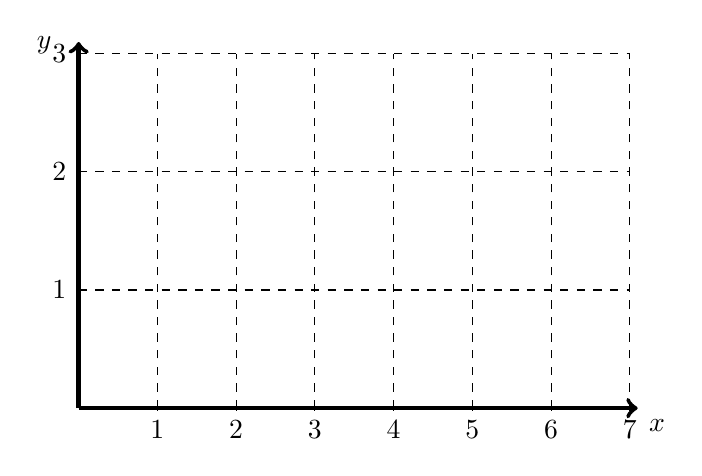
\begin{tikzpicture}[y=1.5cm, x=1.0cm,font=\sffamily]
      \begin{scope}[shift={(0,0)}]
        %% ticks
        \draw[xstep = 1, ystep=1,black,dashed] % very thin,opacity=0.85,
            (0.0, 0.0) grid ( 7.0, 3.0);
        %% axis
        \draw[ultra thick,->] (0,0) -- coordinate (x axis mid) (7.1,0)
             node[anchor = north west] {$x$};

        \draw[ultra thick,->] (0,0) -- coordinate (y axis mid) (0,3.1)
             node[anchor = south east,shift={(-0.2,-0.2)}] {$y$};

        \foreach \y in {1,2,3} {
          \draw (1pt, \y) -- (-1pt,\y) node[anchor = east] {$\y$}; }

        \foreach \x in {1,...,7} {
          \draw (\x,1pt) -- (\x,-1pt) node[anchor =north] {$\x$}; }

      \end{scope}

      \end{tikzpicture}

\item Determine an approximation of the integral
  \begin{eqnarray*}
    \int_1^6 \frac{1}{x} ~ dx
  \end{eqnarray*}
  using a left sided Riemann sum where $\triangle x$=1.
  Make a sketch of the rectangles that are used to approximate the integral using your sketch above.
  Is your approximation too low or too high? (Explain why.)
  \sideNote{Leave your approximation as a sum. Do not evaluate the sum.}

  \vfill

  \item Determine an approximation of the integral
    \begin{eqnarray*}
      \int_1^6 \frac{1}{x} ~ dx
    \end{eqnarray*}
    using a right sided Riemann sum where $\triangle x$=1.
    Make a sketch of the rectangles that are used to approximate the integral using your sketch above.
    Is your approximation too low or too high? (Explain why.)
    \sideNote{Leave your approximation as a sum. Do not evaluate the sum.}

    \vfill

  \end{subproblem}
\end{problem}


\actTitle{The Integral Test}
A glass lens can be used to make it look as if an object appears in different place. An example is shown in the diagram below.
  A lens has a focal length, $f_1$. An object is sitting a distance $s_1$ to the left of the lens, and the resulting image
  appears to be sitting a distance of $s_2$ from the lens.

  \newcommand{\stickFigure}[3]{%
    \begin{scope}[shift={(#1,#2)},y=#3]
      \fill[black] (0,1.0) circle[radius=3pt];       % Draw the head
      \draw[black] (0,1.0) -- (0,.33);               % Draw the body
      \draw[black] (-0.25,0) -- (0,.33) -- (.25,0);  % Draw the legs
      \draw[black] (-.3,0.8) -- (.3,0.8);            % Draw the arms
    \end{scope}
  }
  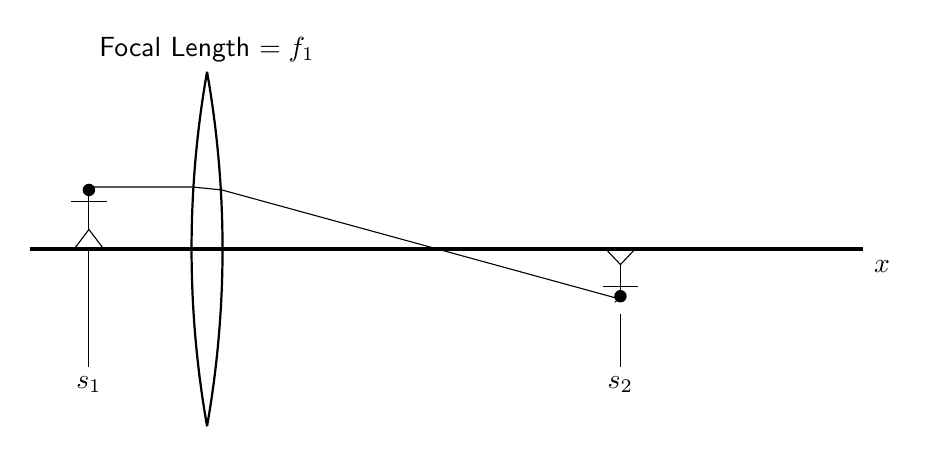
\begin{tikzpicture}[y=1.0cm, x=1.0cm,font=\sffamily,scale=0.75]
      %% axis
      \draw[ultra thick] (-7,0) -- coordinate (x axis mid) (7.1,0)
           node[anchor = north west] {$x$};

      % Draw the lens
      \draw[thick,black] (-4,-3) arc(-10: 10:17.276);
      \draw[thick,black] (-4,-3) arc(190:170:17.276) node[anchor=south] at (-4,3) {Focal Length $ = f_1$};

      % Draw the stick figures
      \stickFigure{-6}{0}{1cm}
      \stickFigure{3}{0}{-0.8cm}

      % Annotate the figure
      \draw[thin,->] (-6,1.05) -- (-4.25,1.05) -- (-3.75,1.0) -- (3,-0.85);
      \draw[thin] (-6,   0) -- (-6,-2) node[anchor=north] {$s_1$};
      \draw[thin] (3,-1.1) -- (3,-2) node[anchor=north] {$s_2$};
    \end{tikzpicture}

    The relationship between the three variables is
    \begin{eqnarray}
      \label{eqn:lensDistOne}
      \frac{1}{s_1} + \frac{1}{s_2} & = & \frac{1}{f_1}.
    \end{eqnarray}
    In this case the lens is convex on both sides, so if the original object is to the left of the lens then $s_1$ is positive.
    If the image is to the right then $s_2$ is positive as well.

    Now suppose that there are two lenses. We start with the same situation as above, but a second lens is added very close to the first lens as shown in the diagram below.
    The location where the object appears, though, has not changed, and the diagram is not correct. The second lens will change the location of the image that is located at $s_2$.
    Because the image from the first lens is to the right of the new convex lens, the distance is negative. Also, we assume that the lenses are close,
    so the image's distance to the second lens is approximately $-s_2$.

    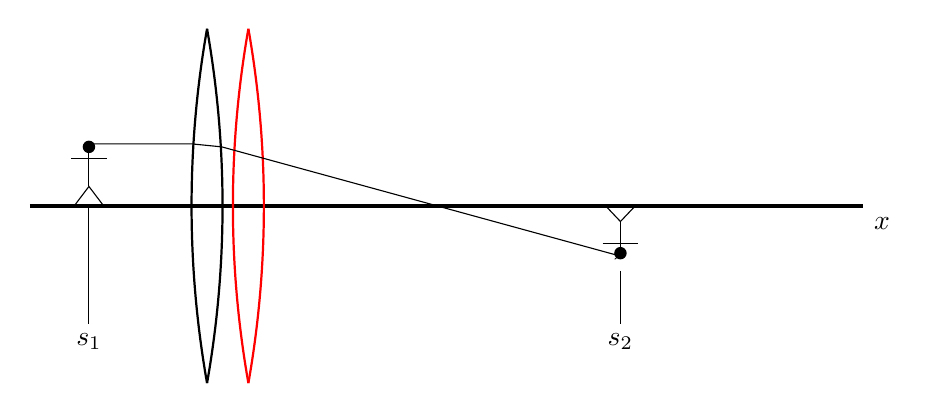
\begin{tikzpicture}[y=1.0cm, x=1.0cm,font=\sffamily,scale=0.75]
        %% axis
        \draw[ultra thick] (-7,0) -- coordinate (x axis mid) (7.1,0)
             node[anchor = north west] {$x$};

        % Draw the first lens
        \draw[thick,black] (-4,-3) arc(-10: 10:17.276);
        \draw[thick,black] (-4,-3) arc(190:170:17.276);
        % Draw the second lens
        \draw[thick,red] (-3.3,-3) arc(-10: 10:17.276);
        \draw[thick,red] (-3.3,-3) arc(190:170:17.276);

        % Draw the stick figures
        \stickFigure{-6}{0}{1cm}
        \stickFigure{ 3}{0}{-0.8cm}

        % Annotate the figure
        % Annotate the figure
        \draw[thin,->] (-6,1.05) -- (-4.25,1.05) -- (-3.75,1.0) -- (3,-0.85);
        \draw[thin] (-6,   0) -- (-6,-2) node[anchor=north] {$s_1$};
        \draw[thin] (3,-1.1) -- (3,-2) node[anchor=north] {$s_2$};
      \end{tikzpicture}

      The distance to where the correct image should be is called $s_3$, and it satisfies
      \begin{eqnarray}
        \label{eqn:lensDistTwo}
        \frac{-1}{s_2} + \frac{1}{s_3} & = & \frac{1}{f_2},
      \end{eqnarray}
      where $f_2$ is the focal length of the second lens.

\clearpage

\begin{problem}
  \item Solve for $\frac{1}{s_2}$ in \ref{eqn:lensDistOne}. Substitute the result into equation \ref{eqn:lensDistTwo} to show that
  \begin{eqnarray}
    \label{eqn:lensDistTwoCombined}
    \frac{1}{s_1} + \frac{1}{s_3} & = & \frac{1}{f_1} + \frac{1}{f_2}.
  \end{eqnarray}

  \vfill
  \vfill

  \item Suppose that a third lens is added. The original image is still located at $s_1$, but the new image for the third lens will be located at $s_4$.
  Assuming that the lens are close we get that the source for the third mirror is located at $-s_3$. Use equation \ref{eqn:lensDistTwoCombined} and the equation for the new lens to show that
  \begin{eqnarray*}
    \frac{1}{s_1} + \frac{1}{s_4} & = & \frac{1}{f_1} + \frac{1}{f_2}. + \frac{1}{f_3}.
  \end{eqnarray*}

    \vfill
    \vfill

  \item What is the pattern? And using these assumptions what will be the relationship after a fourth lens is added?

  \vfill

  \item What will the relationship when there are $n$ lens?

  \vfill

\clearpage

\item Assume that the focal lengths of the lens are increasing, and $f_n=n$. (For example, $f_3=3$.)
What do you get for your series in the previous question?
  \vfill

\item From the pre-class activity, how does this value compare to the integral
\begin{eqnarray*}
  \int^{n+1}_1 \frac{1}{x} ~ dx?
\end{eqnarray*}
\sideNote{Make a sketch of a graph of the function and the corresponding Riemann sum to approximate the integral above.}
\vfill

\item From the pre-class activity, how does this value compare to the integral
\begin{eqnarray*}
  \int^{n}_0 \frac{1}{x} ~ dx?
\end{eqnarray*}
\sideNote{Make a sketch of a graph of the function and the corresponding Riemann sum to approximate the integral above.}
\vfill

\clearpage

\item Determine the value of
  \begin{eqnarray*}
    \lim_{n\rightarrow\infty} \int_1^n \frac{1}{x} ~ dx.
  \end{eqnarray*}
  \vfill

\item Based on your result what can you say about the series
  \begin{eqnarray*}
    \sum_{n=1}^\infty \frac{1}{n}?
  \end{eqnarray*}
  \vfill

\end{problem}


\postClass

\begin{problem}
\item Briefly state two ideas from today's class.
  \begin{itemize}
  \item
  \item
  \end{itemize}
\item Determine which of the following series converges or
  diverges.
  \sideNote{Clearly state your reasoning. The process and
    communication is just as important as the result itself.}
  \begin{subproblem}
    \item $\sum_{n=1}^\infty \frac{1}{n}$
      \vfill
    \item $\sum_{n=0}^\infty \frac{e^n}{1+e^n}$
      \vfill
      \clearpage
    \item $\sum_{n=0}^\infty e^{-n}$
      \vfill
    \item $\sum_{n=0}^\infty \frac{1}{n^2+1}$
      \vfill
  \end{subproblem}
\end{problem}


%=========================================================================
% The comparison test
%=========================================================================
\preClass{Comparing Terms In A Series}

\begin{problem}
  \item We examine the terms in the partial sum given by
  \begin{eqnarray*}
    S_N & = & \sum^N_{n=1} \frac{1}{n} \\
    & = & 1 + \frac{1}{2} + \frac{1}{3} + \frac{1}{4} + \frac{1}{5} + \frac{1}{5} + \frac{1}{6} + \frac{1}{7} + \frac{1}{8} + \cdots + \frac{1}{N}, \\
    & = & \underbrace{1}_{\mathrm{Group~1}} + \underbrace{\frac{1}{2}}_{\mathrm{Group~2}} + \underbrace{\frac{1}{3} + \frac{1}{4}}_{\mathrm{Group~3}}
     + \underbrace{\frac{1}{5} + \frac{1}{6} + \frac{1}{7} + \frac{1}{8}}_{\mathrm{Group~4}} + \cdots
  \end{eqnarray*}
  \begin{subproblem}
    \item Are the numbers in group 1 bigger than or equal to one half?
      \vfill
    \item Are the numbers in group 2 bigger than or equal to one half?
      \vfill
    \item Are the numbers in group 3 bigger than or equal to one half? Briefly xplain why.
    \vfill
    \vfill
    \item Are the numbers in group 4 bigger than or equal to one half? Briefly xplain why.
    \vfill
    \vfill
    \item Write out the numbers that would be in group 5. Are the numbers in group 5 bigger than or equal to one half? Briefly explain why.
    \vfill
    \vfill
    \item  What does this imply about the sequence of partial sums? (Determine a lower bound for the value of $S_{2^{m+1}}$ where $m$ is an integer.)
    \vfill
  \end{subproblem}

\end{problem}


\actTitle{The Comparison Test}
\begin{problem}
  \item Which number is bigger, $\frac{1}{3,000}$ or $\frac{1}{2,500}$. Justify your answer without using a calculator.
    \vspace{1em}
  \item We examine the series
  \begin{eqnarray*}
    \sum^\infty_{n=1} \frac{1}{n^2+1}.
  \end{eqnarray*}
  \begin{subproblem}
    \item Based on your first impression do you think the series will converge or diverge. Briefly give a reason for your suspicians.
    \vfill
    \item Does the series
    \begin{eqnarray*}
      \sum^\infty_{n=1} \frac{1}{n^2}
    \end{eqnarray*}
    converge or diverge? (Fully justify your conclusions.)
    \vfill
    \item Write out the $N$\textsuperscript{th} partial sums for the two series, one above the other. How do the individual terms compare to one another?
      \vfill
    \item What does this imply about the original series?
    \vfill
  \end{subproblem}
  \clearpage

  \item A comparison will be made between the two series
  \begin{eqnarray*}
    \sum^\infty_{n=2} \frac{n}{n^2-1}, & \mathrm{and} &  \sum^\infty_{n=2} \frac{1}{n}.
  \end{eqnarray*}
  \begin{subproblem}
    \item How do the individual terms compare with one another?
    \vfill
    \item What does this imply about the two series? (Hint: Start with the series for which you already know whether or not it converges.)
    \vfill
    \vfill
    \item Write a complete statement that states your conclusion and includes the reasoning you used to justify your conclusion.
    \vspace{2em}
  \end{subproblem}
  \clearpage

\item For each series below state the series that you would use to compare the series. State whether or not the series you will use converges or diverges.
Then state what this implies about the original series.
  \sideNote{Clearly state your reasoning. The process and
    communication is just as important as the result itself.}
  \begin{subproblem}
    \item $\sum_{n=0}^\infty \frac{1}{1+3^n}$
      \vfill
    \item $\sum_{n=1}^\infty \frac{1}{n5^n}$
      \vfill
      \clearpage
    \item $\sum_{n=2}^\infty \frac{1}{n-1}$
      \vfill
    \item $\sum_{n=2}^\infty \frac{n}{n^2+1} $
      \vfill
  \end{subproblem}
\end{problem}


\postClass

\begin{problem}
\item Briefly state two ideas from today's class.
  \begin{itemize}
  \item
  \item
  \end{itemize}
\item
  \begin{subproblem}
    \item
  \end{subproblem}
\end{problem}


%=========================================================================
% Limit Comparison test
%=========================================================================
\preClass{Introduction to the Limit Comparison Test}

\begin{problem}
\item We will examine the series
    \begin{eqnarray*}
      & & \sum^\infty_{n=2} \frac{n^2-1}{n^4+n}.
    \end{eqnarray*}
    \begin{subproblem}
      \item Write out the expression for the first three values in the sequence of partial sums.
      \vfill
      \item Write out the general expression for the $n$\textsuperscript{th} term in the original series above.
        \vfill
      \item What is the order of the polynomial in the numerator?
      \vfill
      \item What is the order of the polynomial in the denominator?
      \vfill
      \item Looking at the denominator, $n^4+n$, as $n$ gets bigger which term grows faster?
      \vfill
    \end{subproblem}
\end{problem}


\actTitle{Limit Comparison Test}
\begin{problem}
  \item We will examine the series
  \begin{eqnarray*}
    \sum^\infty_{n=1} \frac{3n^4 - n^3 + n}{8n^6 + 3n^4 - 1}.
  \end{eqnarray*}
  \begin{subproblem}
      \item Write out the general expression for the $n$\textsuperscript{th} term in the series.
      \vfill
      \item What is the leading order term in the numerator?
      \vfill
      \item What is the leading order term in the denominator?
      \vfill
      \item What is the value of the leading order term in the numerator divided by the leading order term in the denominator?
      \vfill
      \clearpage
      \item If you have a series based on a sum of the terms using the previous expression would it converge or diverge?
      \label{subproblem:limitterm}
      \vfill
      \item Perform the limit ratio test using the series described in part \ref{subproblem:limitterm}.
      \vfill
      \vfill
      \vfill
  \end{subproblem}
  \clearpage
  \item Determine if the series
  \begin{eqnarray*}
    \sum^\infty_{n=0} \frac{3n+1}{4n^2-n+9}
  \end{eqnarray*}
  converges.
  \begin{subproblem}
    \item  Determine the ratio of the leading order terms in the numerator and denominator of the terms being added in the series above.
    \vfill
    \item Determine a series to use for the limit comparison test. Will this new series converge or diverge?
    \vfill
    \item Perform the limit comparison test.  Make sure to provide a complete statement justifying your final conclusion.
    \vfill
    \vfill
    \vfill
  \end{subproblem}

  \clearpage

\item For each series below determine if the series converges or diverges. Include a complete statement in each case justifying your conclusion.
  \begin{subproblem}
    \item $\sum_{n=1}^\infty \frac{5^{n-1}}{3^{n+1}+1}$
      \vfill
    \item $\sum_{n=1}^\infty \frac{6}{n7^n}$
      \vfill
      \clearpage
    \item $\sum_{n=0}^\infty \frac{4}{n^{3.2}} $
      \vfill
    \item $\sum_{n=1}^\infty \frac{\pi^n}{2\cdot 4^{n-1}}$
      \vfill
      \clearpage
  \end{subproblem}
\end{problem}


\postClass

\begin{problem}
\item Briefly state two ideas from today's class.
  \begin{itemize}
  \item
  \item
  \end{itemize}
\item
  \begin{subproblem}
    \item
  \end{subproblem}
\end{problem}

%=========================================================================
% Absolute Convergence and root and ratio tests
%=========================================================================
\preClass{Series With Negative Terms}

\begin{problem}
\item For each series determine if it converges or diverges.
  \begin{subproblem}
  \item
    \begin{eqnarray*}
      & & \sum^\infty_{n=2} \frac{-1}{n^3-1}.
    \end{eqnarray*}
    \vfill
  \item
    \begin{eqnarray*}
      & & \sum^\infty_{n=1} \frac{-2}{\sqrt{n}+1}.
    \end{eqnarray*}
    \vfill
  \end{subproblem}
\end{problem}


\actTitle{Root and Ratio Tests}
\begin{problem}
  \item Determine the first five terms in the sequence of partial sums for the series
  \begin{eqnarray*}
    \sum^\infty_{n=1} \frac{1}{n}.
  \end{eqnarray*}
  \vfill

  \item Determine the first five terms in the sequence of partial sums for the series
  \begin{eqnarray*}
    \sum^\infty_{n=0} \frac{1}{n!}.
  \end{eqnarray*}
  \vfill

  \clearpage

\item Determine whether you should use a comparison, limit comparison,
  root, or ratio test for each series. Do not perform the test just decide
  which one to use. For a comparison or limit comparison state which
  series you would use for the comparison.
  \sideNote{Clearly state your reasoning. The process and
    communication is just as important as the result itself.}
  \begin{subproblem}
    \item $\sum_{n=1}^\infty \frac{1}{\sqrt{n}+5}$
      \vfill
    \item $\sum_{n=0}^\infty \frac{5}{n!}$
      \vfill
    \item $\sum_{n=0}^\infty \frac{2^n}{(n+1)^n} $
      \vfill
      \clearpage
    \item $\sum_{n=1}^\infty \frac{2^{n-1}}{e^{2n}}$
      \vfill
    \item $\sum_{n=0}^\infty \frac{n}{5n^2+3} $
      \vfill
    \item $\sum_{n=1}^\infty \frac{n+1}{2n^9-n}$
      \vfill
  \end{subproblem}
\end{problem}


\postClass

\begin{problem}
\item Briefly state two ideas from today's class.
  \begin{itemize}
  \item
  \item
  \end{itemize}
\item
  \begin{subproblem}
    \item
  \end{subproblem}
\end{problem}


%=========================================================================
% Alternating Series Test
%=========================================================================
\preClass{Increasing Versus Decreasing Terms In A Series}

\begin{problem}
\item Determine if the individual terms in the series
  \begin{eqnarray*}
    & & \sum^\infty_{n=1} \frac{1}{n^2+1}
  \end{eqnarray*}
  are increasing or decreasing.
%    \begin{eqnarray*}
%      & & \sum^\infty_{n=1} \frac{4^n+1}{3^n+1}.
%    \end{eqnarray*}

    \vfill


  \item  Determine the first four terms in each of the sequences below. Express the values as numbers and not a formula of a trigonometric function.
    \begin{subproblem}
      \item $\displaystyle \left\{ \cos\lp n\pi \rp\right\}_{n=0}^\infty$
        \vfill
      \item $\displaystyle \left\{ \sin\lp \frac{(2n+1)\pi}{2}\rp\right\}_{n=0}^\infty$
        \vfill
    \end{subproblem}
\end{problem}


\actTitle{Alternating Series Tests}
\begin{problem}
\item Determine whether or not each of the following series converges
  or diverges. Show all of your work!
  \sideNote{Clearly state your reasoning. The process and
    communication is just as important as the result itself.}
  \begin{subproblem}
    \item $\displaystyle \sum_{n=0}^\infty \frac{(-1)^n}{n^2+1}$
      \vfill
    \item $\displaystyle \sum_{n=1}^\infty \frac{\cos\lp n\pi \rp}{n^2}$
      \vfill
      \clearpage
    \item $\displaystyle \sum_{n=1}^\infty \frac{\sin\lp\frac{(2n+1)\pi}{2}\rp}{n} $
      \vfill
    \item $\displaystyle \sum_{n=1}^\infty \frac{\cos\lp 2n\pi \rp}{n^2}$
      \vfill
  \end{subproblem}
\end{problem}


\postClass

\begin{problem}
\item Briefly state two ideas from today's class.
  \begin{itemize}
  \item
  \item
  \end{itemize}
\item
  \begin{subproblem}
    \item
  \end{subproblem}
\end{problem}

%=========================================================================
% Review of Sequences and Series
%=========================================================================
\preClass{Sequence and Series}
\begin{problem}
    \item Make a list of all of the tests we can use to determine if a series converges or diverges.
\end{problem}

\actTitle{Review of Sequences and Series}
\begin{problem}
\item What is a sequence?
  \vfill
\item What is a series?
  \vfill

\item  What is a geometric series, and what are the conditions for a geometric series to converge?
  \vfill

\item  What is a $p$-series, and what are the conditions for a $p$-series to converge?
  \vfill

  \item  What is a telescoping series, and what are the conditions for a telescoping series to converge?
    \vfill

  \clearpage

  \item The different tests that we have covered are given in the flow chart below.
        Next to each test write out the conditions and steps associated with the test.

  \tikzstyle{known} = [rectangle, rounded corners, minimum width=3cm, minimum height=1cm,text centered, draw=black, fill=green!30]
  \tikzstyle{test}  = [rectangle, rounded corners, minimum width=3cm, minimum height=1cm,text centered, draw=black, fill=blue!30]
  \tikzstyle{root}  = [rectangle, rounded corners, minimum width=3cm, minimum height=1cm,text centered, draw=black, fill=red!30]
  \tikzstyle{arrow} = [thick,->,>=stealth]
  \begin{tikzpicture}[node distance = 3cm]
    % First Draw the nodes
    \node [root] (series) {Given $\sum^\infty_{n=0}a_n$.};
    \node [root, below of=series,yshift=1cm] (root) {Is this a known series?};
    \node [known, below of=root, xshift=-5cm] (geometric) {Geometric Series};
    \node [known, below of=geometric] (pseries) {$p$-Series};
    \node [known, below of=pseries] (telescoping) {Telescoping Series};
    \node [test, below of=root] (alternating) {Alternating Series};
    \node [test, below of=root,xshift=5cm] (absconv) {Absolutely Convergent?};
    \node [test, below of=absconv] (integral) {Integral Test};
    \node [test, below of=integral] (comparison) {Comparison Test};
    \node [test, below of=comparison] (limitComp) {Limit Comparison Test};
    \node [test, below of=limitComp] (rootTest) {Root Test};
    \node [test, below of=rootTest] (ratio) {Ratio Test};
    % Next draw the arrows
    \draw [arrow] (series) -- (root);
    \draw [arrow] (root) -- node[anchor=east] {yes} (geometric);
    \draw [arrow] (geometric) -- (pseries);
    \draw [arrow] (pseries) -- (telescoping);
    \draw [arrow] (root) -- node[anchor=east,yshift=-0.5cm] {Alternating?} (alternating);
    \draw [arrow] (root) -- node[anchor=west,xshift=0.1cm] {Other?} (absconv);
    \draw [arrow] (absconv) -- (integral);
    \draw [arrow] (integral) -- (comparison);
    \draw [arrow] (comparison) -- (limitComp);
    \draw [arrow] (limitComp) -- (rootTest);
    \draw [arrow] (rootTest) -- (ratio);
  \end{tikzpicture}

  \clearpage

  \item For each series below determine whether or not the series converges. Justify your answers.

  \begin{subproblem}
  \item $\displaystyle \sum^\infty_{n=0} \frac{2^n}{n!}$
    \vfill
  \item $\displaystyle \sum^\infty_{n=0} \frac{3n}{5n^2+1}$
    \vfill
  \item $\displaystyle \sum^\infty_{n=1} \frac{\lp\frac{1}{3}\rp^n}{4n-1}$
    \vfill
    \clearpage
  \item $\displaystyle \sum^\infty_{n=0} n\cdot\frac{1}{6^n}$
    \vfill
  \item $\displaystyle \sum^\infty_{n=1} \lp\frac{1+n}{2n}\rp^n$
    \vfill
  \item $\displaystyle \sum^\infty_{n=1} \frac{\arctan(n)}{1+n^2}$
    \vfill
  \end{subproblem}

\end{problem}

\postClass

\begin{problem}
\item Briefly state two ideas from today's class.
  \begin{itemize}
  \item
  \item
  \end{itemize}
\item
  \begin{subproblem}
    \item
  \end{subproblem}
\end{problem}


%========================================================================\=
% Power Series
%=========================================================================
\preClass{Power Series}

\begin{problem}
\item Evaluate each of the following functions at $x=1$.
  \begin{subproblem}
  \item
    \begin{eqnarray*}
      f_3(x) & = & 1 + x + \frac{x^2}{2!} + \frac{x^3}{3!}.
    \end{eqnarray*}
    \vfill
  \item
    \begin{eqnarray*}
      f_4(x) & = & 1 + x + \frac{x^2}{2!} + \frac{x^3}{3!} + \frac{x^4}{4!}.
    \end{eqnarray*}
    \vfill
  \item
    \begin{eqnarray*}
      f_5(x) & = & 1 + x + \frac{x^2}{2!} + \frac{x^3}{3!} +
                   \frac{x^4}{4!} + \frac{x^5}{5!}.
    \end{eqnarray*}
    \vfill
  \item
    \begin{eqnarray*}
      f_6(x) & = & 1 + x + \frac{x^2}{2!} + \frac{x^3}{3!} +
                   \frac{x^4}{4!} + \frac{x^5}{5!} + \frac{x^6}{6!}.
    \end{eqnarray*}
    \vfill
  \item
    \begin{eqnarray*}
      g(x) & = & e^x.
    \end{eqnarray*}
    \vfill
  \end{subproblem}
\end{problem}


\actTitle{Power Series}
\begin{problem}
\item Determine the radius of convergence for each of the series
  below. Show all of your work!  \sideNote{Clearly state your
    reasoning. The process and communication is just as important as
    the result itself.}
  \begin{subproblem}
    \item $\displaystyle \sum_{n=0}^\infty \frac{x^n}{2^n}$
      \vfill
    \item $\displaystyle \sum_{n=0}^\infty \frac{(x-3)^n}{2^n}$
      \vfill
      \clearpage
    \item $\displaystyle \sum_{n=1}^\infty \frac{x^n}{n} $
      \vfill
    \item $\displaystyle \sum_{n=0}^\infty \frac{x^n}{n!} $
      \vfill
  \end{subproblem}
  \clearpage
  \item Determine the formula for the tangent line for each of the functions given below at the given point.
  \begin{subproblem}
    \item $\displaystyle f(x)=e^x$ at $x=0$.
    \vfill
    \item $\displaystyle f(x)=\sin(x)$ at $x=\pi$.
    \vfill
  \end{subproblem}
\end{problem}


\postClass

\begin{problem}
\item Briefly state two ideas from today's class.
  \begin{itemize}
  \item
  \item
  \end{itemize}
\item
  \begin{subproblem}
    \item
  \end{subproblem}
\end{problem}


%=========================================================================
% Taylor Series
%=========================================================================
\preClass{Taylor Series}

Answer the three questions before class and show your work.

\begin{problem}
\item We will construct an approximation of the function
  \begin{eqnarray*}
    f(x) & = & \cos(x).
  \end{eqnarray*}
  The approximation is a polynomial that is defined by
  \begin{eqnarray*}
    p(x) & = & a x^2 + b x + c,
  \end{eqnarray*}
  where $a$, $b$, and $c$ are constants.
  Determine values of $a$, $b$, and $c$ so that $p_2(\pi)=f(\pi)$,
  $p_2'(\pi)=f'(\pi)$, and $p_2''(\pi)=f''(\pi)$.
  \vfill

  \clearpage

\item Make a sketch of the functions, $p_2(x)$ and $f(x)$, for $x$ from $\frac{\pi}{2}$ to
  $\frac{3\pi}{2}$. Use your calculator to plot the two functions and
  sketch the result.

  \vfill

\item A function is defined to be
  \begin{eqnarray*}
    h(x) & = & a (x-\pi)^2 + b (x-\pi) + c.
  \end{eqnarray*}
  Expand the quadratic term (FOIL) and express the function as a
  polynomial of degree two.

  \vspace{5em}


\end{problem}


\actTitle{Taylor Series}
\begin{problem}
\item Suppose we want to construct an approximation of the function
  \begin{eqnarray*}
    f(x) & = & \cos(x).
  \end{eqnarray*}
  To do so a polynomial is defined to be
  \begin{eqnarray*}
    p_2(x) & = & a (x-\pi)^2 + b (x-\pi) + c,
  \end{eqnarray*}
  where $a$, $b$, and $c$ are constants.  Determine
  values of $a$, $b$,  and $c$ so that the
  polynomial is the same value and its first through second
  derivatives are the same as those of the function $f(x)=\cos(x)$ when
  $x=\pi$.
  \vfill

\item Make a sketch of the functions, $p_2(x)$ and $f(x)$, from the
  previous question. Plot the function for $x$ from $\frac{\pi}{2}$ to
    $\frac{3\pi}{2}$.

  \vspace{5em}


  \clearpage

\item A polynomial is defined to be
  \begin{eqnarray*}
    p_4(x) & = &  a_0 + a_1 (x-\pi) +  a_2 (x-\pi)^2 +  a_3 (x-\pi)^3 +  a_4 (x-\pi)^4,
  \end{eqnarray*}
  where $a_4$, $a_3$, $a_2$, $a_1$ and $a_0$ are constants.  Determine
  values of $a_4$, $a_3$, $a_2$, $a_1$ and $a_0$ so that the
  polynomial is the same value and its first through fourth
  derivatives are the same as those of the function $f(x)=\cos(x)$ when
  $x=\pi$.

  \vfill

\item Make a sketch of the functions, $p_2(x)$, $p_4(x)$ and $f(x)$,
  from the previous questions. Plot the function for $x$ from $\frac{\pi}{2}$ to
    $\frac{3\pi}{2}$.

  \vspace{5em}


\end{problem}


\postClass

\begin{problem}
\item Briefly state two ideas from today's class.
  \begin{itemize}
  \item
  \item
  \end{itemize}
\item
  \begin{subproblem}
    \item
  \end{subproblem}
\end{problem}


\preClass{Taylor Series}

\begin{problem}
\item Determine the second and the third order Taylor polynomials for
  $f(x)=e^x$ centered at $x=0$. Make a sketch of the two polynomials
  and the original function for $-2 < x < 2$.

  \vfill

  \clearpage

\item Determine the radius of convergence and the values of $x$ for
  which the series
  \begin{eqnarray*}
    p(x) & = & \sum^\infty_{n=1} \frac{x^n}{n}
  \end{eqnarray*}
  converge.

  \vfill

\end{problem}


\actTitle{Taylor Series}
\begin{problem}
\item Determine the Taylor polynomial for $f(x)=e^x$ centered at $x=0$
  and determine the general form for the polynomial's coefficient.
  Make plot of the original function and the first, second, and third Taylor polynomial.

  \vfill


  \clearpage

\item Determine the radius of convergence and the values of $x$ for
  which the series in the previous question converge.

  \vfill


  \clearpage

\item Determine the derivative of $e^x$, and determine the derivative of the Taylor
polynomial of $e^x$ centered at $x=0$.
  \vfill

  \clearpage

  \item Determine the anti-derivative of $e^x$, and determine the anti-derivative of the Taylor
  polynomial of $e^x$ centered at $x=0$.
    \vfill

\end{problem}


\postClass

\begin{problem}
\item Briefly state two ideas from today's class.
  \begin{itemize}
  \item
  \item
  \end{itemize}
\item
  \begin{subproblem}
    \item
  \end{subproblem}
\end{problem}




%%% Local Variables:
%%% mode: latex
%%% TeX-master: t
%%% End:
